% vim:foldmethod=marker:fmr=<<<,>>> spell nowrap
\documentclass{article}

\usepackage[utf8]{inputenc}
% \usepackage[T1]{fontenc}
\usepackage[total={6.2in, 8in}]{geometry}

\usepackage{amsmath, amsthm, amssymb,amsfonts, mathtools}
\usepackage{graphicx}
\usepackage{float}
\usepackage[percent]{overpic} %writing over pictures
\usepackage{xcolor}
\usepackage{appendix}

\usepackage{mdframed}
\usepackage[colorlinks,urlcolor=blue]{hyperref}
\usepackage{verbatim}
%\usepackage{fancyvrb}
\usepackage{minted}
\renewcommand{\MintedPygmentize}{pygmentize}
\usepackage[ruled,linesnumbered]{algorithm2e}
\setlength{\algomargin}{10pt}
\usepackage[normalem]{ulem}
\usepackage{varwidth}

\usepackage{biblatex}
\addbibresource{main.bib}

\usepackage{listings}
\usepackage{tikz-cd}
\usepackage{enumitem}
\usepackage{tikzsymbols}

\lstset{
basicstyle=\small\ttfamily,
columns=flexible,
breaklines=true
}
\usepackage{tikz}

\setlength{\parindent}{0pt}

\newcommand{\ket}[1]{\left|{#1}\right\rangle}
\newcommand{\bra}[1]{\left\langle{#1}\right|}
\newcommand{\BS}{\backslash}

\newcommand{\CLR}[2]{\begingroup\color{#1}#2\endgroup}
\newcommand{\R}[1]{\begingroup\color{red}#1\endgroup}
\newcommand{\G}[1]{\begingroup\color{green}#1\endgroup}
\newcommand{\B}[1]{\begingroup\color{blue}#1\endgroup}
\newcommand{\Y}[1]{\begingroup\color{yellow}#1\endgroup}
\newcommand{\N}{\mathbb{N}}
\newcommand{\Z}{\mathbb{Z}}
\newcommand{\Rational}{\mathbb{R}}
\newcommand{\Rat}{\mathbb{R}}
\newcommand{\Pow}{\mathbb{P}}

\newcommand{\vsp}[0]{\vspace*{10pt}\par}
\newcommand{\tcite}[1]{\textit{(\citefield{#1}{year}, \citeauthor{#1})}\:\textit{``\citefield{#1}{title}''}\:\cite{#1}}
\newcommand{\exercise}[1]{\subsubsection*{#1}}
\newcommand{\ans}[0]{\vsp\textbf{Answer: }\vsp}
\newcommand{\problem}[0]{\vsp\textbf{Problem: }\vsp}
\newcommand{\unsure}[0]{TODO: (\textbf{unsure}) }

\newcommand{\JProg}{\mathbb{J}}
\newcommand{\AST}{\mathbb{AST}}
\newcommand{\TNET}{\mathbb{TNET}}
\newcommand{\CV}{\Rational^N}
\newcommand{\U}[1]{{\underline{#1}}}
\newcommand{\REM}[1]{\tcp*{\parbox[t]{2.0in}{\raggedright #1}}}

\newcommand{\toto}[0]{\begin{array}{c}\rightarrow \\[-1.9ex]\rightarrow\end{array}}

\newcommand{\ei}{\item}
\newcommand{\es}{\begin{enumerate}[label=(\alph*)]\ei}
\newcommand{\ee}{\end{enumerate}}

\newcommand{\ls}{\begin{itemize}\item}
\newcommand{\li}{\item}
\renewcommand{\le}{\end{itemize}}

% Define \set{} command. TODO: Looks too complicated!
\DeclarePairedDelimiterX{\set}[1]{\{}{\}}{\setargs{#1}}
\NewDocumentCommand{\setargs}{>{\SplitArgument{1}{;}}m}
{\setargsaux#1}
\NewDocumentCommand{\setargsaux}{mm}
{\IfNoValueTF{#2}{#1} {#1\,\delimsize|\,\mathopen{}#2}}%{#1\:;\:#2}

% Generic environment for code snippets
\newenvironment{codeverbatim}
  {\VerbatimEnvironment
   \begin{minted}[autogobble,breaklines,fontsize=\footnotesize]{latex}}
  {\end{minted}}
\BeforeBeginEnvironment{codeverbatim}{\begin{mdframed}[nobreak=true,frametitle=\tiny{Source}]}
\AfterEndEnvironment{codeverbatim}{\end{mdframed}}

% LitREPL-compatible environment for code snippets
\newenvironment{python}
  {\VerbatimEnvironment
   \begin{minted}[autogobble,breaklines,fontsize=\footnotesize]{python}}
  {\end{minted}}
\BeforeBeginEnvironment{python}{\begin{mdframed}[nobreak=true,frametitle=\tiny{IPython}]}
\AfterEndEnvironment{python}{\end{mdframed}}

\newenvironment{ai}
  {\vsp\textbf{User:}\vsp}
  {}
\newenvironment{airesult}
  {\vsp\textbf{AI:}\vsp}
  {}
% \newenvironment{ai}
%   {\VerbatimEnvironment
%    \begin{minted}[autogobble,breaklines,fontsize=\footnotesize]{text}}
%   {\end{minted}}
% \BeforeBeginEnvironment{ai}{\begin{mdframed}[nobreak=true,frametitle=\tiny{AI}]}
% \AfterEndEnvironment{ai}{\end{mdframed}}

% LitREPL-compatible environment for code results
\newenvironment{result}
  {\VerbatimEnvironment
   \begin{minted}[autogobble,breaklines,fontsize=\footnotesize]{text}}
  {\end{minted}}
\BeforeBeginEnvironment{result}{\begin{mdframed}[nobreak=true,frametitle=\tiny{Result}]}
\AfterEndEnvironment{result}{\end{mdframed}}

% LitREPL-compatible command for inline code results
\newcommand{\linline}[2]{#2}
\newcommand{\st}[1]{\sout{#1}}
\renewcommand{\t}[1]{\texttt{#1}}



\setcounter{secnumdepth}{4}
% \RedeclareSectionCommand[runin=false,afterskip=0pt,afterindent=false]{paragraph}

\title{Solutions for Category Theory for Scientists by David Spivak}
\author{Sergei Mironov}

\begin{document}

\maketitle

\tableofcontents

\section{Introduction}

The book \tcite{Spivak2013CategoryTF}.

% \setcounter{section}{2}
\section{The Category of Sets}

\exercise{2.3.3.1}

Create an olog for human nuclear biological families that includes the concept of person, man,
woman, parent, father, mother, and child. Make sure to label all the arrows, and make sure each
arrow indicates a valid aspect in the sense of Section 2.3.2.1. Indicate with check-marks the
diagrams that are intended to commute. If the 2-dimensionality of the page prevents a check-mark
from being unambiguous, indicate the intended commutativity with an equation.

\ans

\begin{center}
% https://tikzcd.yichuanshen.de/#N4Igdg9gJgpgziAXAbVABwnAlgFyxMJZARgBoAGAXVJADcBDAGwFcYkQ0YAnOAkAX1LpMufIRTlSxanSat2AW3qFBw7Hj4oATFJkMWbRCADuEJSqEcRG8SVJa9cwx3pcYYHAMsZ1YopIBmRwN2ADN6HAALbi81UU1kHSCafXkjBQgomNUrXwSyABZgtJAAY0isRigBGRgoAHN4IlBQrjMkMhAcCCRJEEZ6ACMYRgAFaz8jRhhQzxSndiwEHNb2xB0unsQ+1OclkBoB4bGJzX6ZzxW2hSQCmm6O+ZCjfau1gFZ7rY3dxYRDoYjcZ5cQgLhYeqRS6WVY3RB3TZIAJPEqvGHXJCfRGIZGyZ4gfYA47A+Kg8GQ6EtDGILEPRAANnu9Eq7EgYDYKOckXo-36gJOIPY5KhsRAsNuXyQjLxJW5vKOQNOZIhIrecNxdOlvyMctF4pxku2nL+Bz5xKVQpVlLF1OldL6wzA1UQAFoAOydbUE+X8kk2S0U01wCqzJBafiUfhAA
\begin{tikzcd}
                                                            & person                                                  &                                                               \\
man \arrow[ru, "is"]                                        &                                                         & woman \arrow[lu, "is"]                                        \\
                                                            & parent \arrow[dd, "has"] \arrow[uu, "is"']              &                                                               \\
father \arrow[uu, "is"] \arrow[ru, "is"] \arrow[rd, "has"'] &                                                         & mother \arrow[uu, "is"'] \arrow[lu, "is"'] \arrow[ld, "has"'] \\
                                                            & child \arrow[uuuu, "is"', bend right=90, shift right=18] &
\end{tikzcd}
\end{center}

Commutative square examples:
\begin{itemize}
\item "parent is person" $\circ$ "mother is parent" $=$ "woman is person" $\circ$ "mother is woman"
\item "mother has child" $=$ "parent has child" $\circ$ "mother is parent"
\item "child is person" $\circ$ "parent has child" $\ne$ "parent is person"
\end{itemize}

\setcounter{subsection}{3}
\subsection{Products and coproducts}

\exercise{2.4.1.4}
How many elements does the $\set{a,b,c,d} * \set{1,2,3}$ have?
\ans
12

\exercise{2.4.1.8}
\ans
(a) No, because $a(b + c) \neq (a+b)c$.
\vsp
(b) No, because $x*0 \neq x$.
\vsp
(c) Yes.

\exercise{2.4.1.15}

(a) Let $X$ and $Y$ be sets.. construct the "swap map" $s:(X \times Y)\to(Y \times X)$
\ans
$s:(X \times Y)\to(Y \times X) = (,)\circ\langle\pi_2,\pi_1\rangle$

Note: we used angle brackets. Is it really correct?

\vsp
(b) Can you prove that $s$ is a isomorphism using only the universal property for product?

Note: $(f:X \to Y)$ is an isomorphism if $\exists (g:Y \to X): g \circ f = id_X \land f \circ g =
id_Y$

Note: diagram $(f,g,h)$ commutes if $f \circ g = h$
\ans

In universal property of products, put $A$ equal to $Y \times X$ and get $\exists !
g:(Y \times X)\to(X \times Y)$. In a similar way, we have $\exists! s:(X \times Y)\to(Y \times X)$.
We need to show that $g \circ s = id_{(X \times Y)}$ and $s \circ g = id_{(Y\times X)}$.

On the following diagram,

% https://tikzcd.yichuanshen.de/#N4Igdg9gJgpgziAXAbVABwnAlgFyxMJZARgBoAmAXVJADcBDAGwFcYkQBBAAgB0e8AtvC4AhEAF9S6TLnyEUZAAzU6TVu259BwsZOnY8BIuVLEVDFm0QhdUkBgNyii0+bVXOElTCgBzeESgAGYAThACSC4gOBBIZCCM9ABGMIwACjKG8iAhWL4AFjggNBbq1nwwAB5YcDhwAIRBEnah4ZE0MUgmqpbsfGhYAPrkxQnJqRmORta5BUV6IK0RiFGdiADMJe59PAODxM3BYcvxa5s9ZSD9Qwc0iSnpmU4zeYWHi8dxHbGI3aUe12GXnEQA
\begin{tikzcd}
  & A \times B \arrow[ld, "\pi_1"'] \arrow[rd, "\pi_2"]                           &   \\
A &                                                                               & B \\
  & A \times B \arrow[uu, "\exists!id"'] \arrow[ru, "\pi_2"'] \arrow[lu, "\pi_1"] &
\end{tikzcd}

$id = id_{(A \times B)}$ - is the unique identity function. By combining diagrams for $f$ and $g$ we
reduce the $g \circ f$ to the similar case.

\exercise{2.4.2.4}

Would you say that a phone is the coproduct of a \texttt{cellphone} and a \texttt{landline phone}?

\ans
Yes, until we consider other types of phones besides cell- and landline ones.

\exercise{2.4.2.10}

Write the universal property for coproduct in terms of a relationship between
$Hom_{Set}(X,A)$, $Hom_{Set}(Y,A)$ and $Hom_{Set}(X \sqcup Y, A)$.

\ans

$Hom_{Set}(X,A) \times Hom_{Set}(Y,A) \cong Hom_{Set}(X \sqcup Y, A)$

\exercise{2.4.2.13}

TODO

\exercise{2.4.2.14}

TODO


\subsection{Finite limits in Set}

\exercise{2.5.1.2}

\ans $X \times_{Z} Y = \set{(x_1,z_1,y_1), (x_2,z_2,y_2), (x_2,z_2,y_4), (x_3,z_2,y_2),
(x_3,z_2,y_4)}$


\exercise{2.5.1.3}

(a)
\ans Let $X = \set{\Y{1},\R{2},\B{3},\Y{4},\R{5}}; Y = \set{\Y{a},\B{b},\R{c}};$ where
$C = \set{\R{R},\B{B},\Y{Y}}$ \vsp We have:
$X \times_C Y = \set{\Y{1a},\Y{4a},\R{2c},\R{5c},\B{3b}}$

(b)
TODO (obvious).

\exercise{2.5.1.5}

(a) Suppose that $Y = \emptyset$; what can you say about $X \times_Z Y$ ?
\ans $X \times_Z Y = \emptyset$ \vsp

(b) $Z = {1}$; what can you say about $X \times_Z Y$ ?
\ans $\forall X,Y : X \times_Z Y \cong X \times Y$

\exercise{2.5.1.6}

.. Aristotelian space and time ..

$S = R^3;\quad T = R;\quad Y = S \times T;\quad g1 : Y \to S ;\quad g2 : Y \to S$ where $g1,g2$
projects space-time to its components. $X = \set{1};\quad f_1 : X \to S;\quad f_2 : X \to T$ is a
set of one element and its space-time projections.

\vsp
(a) What is the meaning of

\begin{minipage}[t]{0.45\textwidth}
\[
\begin{tikzcd}
W_1 \arrow[r] \arrow[d] & Y \arrow[d,"g_1"] \\
X \arrow[r,"f_2"] & S
\end{tikzcd}
\]
\end{minipage}
\quad
\begin{minipage}[t]{0.45\textwidth}
\[
\begin{tikzcd}
W_2 \arrow[r] \arrow[d] & Y \arrow[d,"g_2"] \\
X \arrow[r,"f_2"] & S
\end{tikzcd}
\]
\end{minipage}

\ans $1$ is associated with its time and space. $W_1$ yields time points of $Y$ corresponding
to $1$'s position. $W_2$ yields the space points corresponding to $1$'s time.

\vsp
(b) Interpret the sets in terms of the center of mass of MIT at the time of its founding.

\ans \unsure Is it just the MIT-relative space and time points?

\exercise{2.5.1.10}

.. Appropriate or misleading olog labels ..

\ans
(a) a person whose favorite color is blue - OK
\vsp
(b) a dog whose owner is a woman - OK
\vsp
(c) a good fit - Nope. We would say that a good fit requires less or equal width.

\exercise{2.5.1.11}

(a) Consider your olog from Exercise 2.3.3.1. Are any of the commutative
squares there actually pullback squares?

\ans
Yes, for example: "father" $=$ "man" $\times_{person}$ "parent"

\begin{center}
\begin{tikzcd}
\fbox{father} \arrow[r, "is"] \arrow[d, "is"] & \fbox{man} \arrow[d,"is"] \\
\fbox{parent} \arrow[r,"is"]                  & \fbox{person}
\end{tikzcd}
\end{center}

(b) Now use ologs with products and pullbacks to define what a brother is and
what a sister is:

\ans

\begin{center}
% https://tikzcd.yichuanshen.de/#N4Igdg9gJgpgziAXAbVABwnAlgFyxMJZABgBpiBdUkANwEMAbAVxiRACMAnCHACxk4gAvqXSZc+QigCM5KrUYs2AY15YGUYaJAZseAkTLT59Zq0QgAtnUIixeyUVnHqppRYyWt9iQZmkAJhNFcx0BOAM7HXF9KWQA0hcFMzYAHVTgABV0oW9ohz94wOCUi3Ss0gAxHOF5GCgAc3giUAAzbi9EAGZqHAgkABZXELTUtCwAfWk89ohOnpA+pABWYdKQdPGJgJmOld7+xAA2NfcQLE0o2c6hxcOT5LOwCeBVXKu9xDI7pFlH0KwCA+cyQ3yWiAS-zYgN2IIhByQCzcoTQsM6f3BSJGHlqQiAA
\begin{tikzcd}
brother \arrow[r, "is"] \arrow[d, "is"] & child \arrow[d, "p"]                      &                       \\
man \arrow[r, "p"]                      & pom \arrow[d, "\pi_1"] \arrow[r, "\pi_2"] & \{T\} \arrow[d, "id"] \\
                                        & person \arrow[r, "n_{ch}"]                & {\{T,F\}}
\end{tikzcd}
\end{center}

where: $pom$ stands for "parent of many", $p$ is "has as parent" and $n_{ch}$
is "number of children"

\exercise{2.5.1.13}

Pullback diagram in which the fiber product is isomorphic to the preimage of $y \in Y$.

\ans

\begin{center}
% https://tikzcd.yichuanshen.de/#N4Igdg9gJgpgziAXAbVABwnAlgFyxMJZABgBpiBdUkANwEMAbAVxiRAE0A9YAWgEYAvgB0heALbwABHwD6ATxADS6TLnyEUfclVqMWbWQqUrseAkTJ8d9Zq0QgAGouUgMp9US1XqN-ffaKOjBQAObwRKAAZgBOEGJIWiA4EEgAzD56diBYUM5RsfGIAEzUyWkZtmyReSAxcUhkSSmIib5ZImhYMkU1dYWNZcUVfiAdXXyBAkA
\begin{tikzcd}
Y^{-1} \times \set{y} \arrow[r, "\pi_2"] \arrow[d, "\pi_1"] & \set{y} \arrow[d, "id"] \\
X \arrow[r, "f"]                                            & Y
\end{tikzcd}
\end{center}

\exercise{2.5.1.15}

Create an olog whose underlying shape is a commutative square. Now add the
fiber product so that the shape is the same as that of Diagram (2.32). Assign
English labels to the projections and to the dotted map A, such that these
labels are as canonical as possible.

\ans

\unsure

The general impression is the following:
\begin{itemize}
  \item The commutative square can be visualized as a pyramid in a 3D space.
  \item The pullback corresponds to a 2D plane with two axes.
  \item The pullback over one-element set corresponds to a 2D plane with two orthogonal axes.
  \item The projections $\pi_1$ and $\pi_2$ play the role of parallel
        projections from a point in the plane to its axes.
  \item The map $A \to (D \times_P W)$ acts as a projection from a point in 3D space to the plane.
\end{itemize}

\begin{center}
% https://tikzcd.yichuanshen.de/#N4Igdg9gJgpgziAXAbVABwnAlgFyxMJZARgBpiBdUkANwEMAbAVxiRAAUB1AEQHkQAvqXSZc+QigAMpAExVajFm26DhIDNjwEiM2fPrNWiEJ1UjN4omQDM+xUY4wATnG1DzY7SjKS7htjz8AvIwUADm8ESgAGZOEAC2SAAs1DgQSGQgAEYwYFBIALTW0gr+xgA65WhYAPrEZiCxCcmp6Yi62bn5iMXUBkoVVbUyINQMdDkM7KJaEiBOWGEAFjgNTYmImWlI1u6NcRsd2z1760glx5n9DtUAxjX5pwfnrUgd45PTFl7ziyujpQG6iw92AAHcBGtnogLm0UoCbiCasA0HQsE5IcEBEA
\begin{tikzcd}
             & \fbox{($D \times_P W$) \text{woman dog owner}} \arrow[ldd, "\pi_1", bend right] \arrow[rdd, "\pi_2"', bend left]        &              \\
             & \fbox{(A)\begin{varwidth}{\textwidth} blond woman \\ dog owner \end{varwidth}} \arrow[ld, "has"] \arrow[rd, "is"'] \arrow[u, "\langle\text{has, is} \rangle"] &              \\
\fbox{(D) dog} \arrow[rd] &                                                                                        & \fbox{(W) woman} \arrow[ld] \\
             & \fbox{(P) person}                                                                                   &
\end{tikzcd}
\end{center}

\exercise{2.5.1.18}

(a) Create an olog that defines two people to be 'of approximately the same
height' if and only if their height difference is less than half an inch, using
a pullback.

\ans

\begin{center}
% https://tikzcd.yichuanshen.de/#N4Igdg9gJgpgziAXAbVABwnAlgFyxMJZABgBpiBdUkANwEMAbAVxiRAEEQBfU9TXfIRRkAjFVqMWbAELdeIDNjwEiI8uPrNWiEAGE5fJYNWkx1TVJ0ARAwv7KhyAEzrzk7SACitxQJUoXMwktNgAxbnEYKABzeCJQADMAJwgAWyQyEBwIJCceRJT0xBcsnMQAFnyQZLSkcupspABWKpqigGYGspb5NqQ1UqR21sLcrqGR2sRMxsQRLgouIA
\begin{tikzcd}
  \set{((p_1,p_2),\Delta)|p_1,p_2 \in \text{people}, \Delta \in \Rational} \arrow[r, "\pi_2"] \arrow[d, "\pi_1"] & \set{\Delta|-0.5 < \Delta < 0.5} \arrow[d, "is"] \\
  \fbox{\text{pair of people}} \arrow[r, "h_2 - h_1"]           & \Rational
\end{tikzcd}
\end{center}

(b) In the same olog, make a box for those people whose height is approximately
the same as a person named 'The Virgin Mary'. You may need to use images.

\ans

\begin{center}
% https://tikzcd.yichuanshen.de/#N4Igdg9gJgpgziAXAbVABwnAlgFyxMJZABgBpiBdUkANwEMAbAVxiRAEEQBfU9TXfIRRkAjFVqMWbAELdeIDNjwEiI8uPrNWiEAGE5fJYNWkx1TVJ0ARAwv7KhyAEzrzk7SACitxQJUoXMwktNgAxbnEYKABzeCJQADMAJwgAWyQyEBwIJCceRJT0xBcsnMQAFnyQZLSkcupspABWKpqigGYGspb5NqQ1UqR21sLcrqGR2sRMxsQRLgouIA
\begin{tikzcd}
  \fbox{\text{people of approx Virgin Mary height}} \ar[r, "\pi_2"] \ar[d, "\pi_1"] & \set{((p_1,p_2),\Delta)|...} \arrow[r, "\pi_2"] \arrow[d, "\pi_1"] & \set{\Delta|-0.5 < \Delta < 0.5} \arrow[d, "is"] \\
  \set{(\fbox{The Virgin Mary},p_2)|p_2 \in \text{people}} \ar[r, "is"] & \fbox{\text{pair of people}} \arrow[r, "h_2 - h_1"]           & \Rational
\end{tikzcd}
\end{center}

\unsure We did not use images, despite the textbook suggestion.

\exercise{2.5.1.19}

Let $W = X \times_Z Y$ and $W' = X' \times_{Z'} Y'$, and form the diagram
to the right. Use the universal property of fiber products to construct a map
$W \to W'$ such that all squares commute

\ans

Let $WX = \pi_1$, $WY = \pi_2$, $W'X' = \pi_1'$, $W'Y' = \pi_2'$.  Define $f: W
\to W' = (x,y)_z \mapsto (XX'(x),YY'(y))_{ZZ'(z)}$. We want to show that it
makes $WW'Y'Y$ to commute. Indeed, $\pi_2' \circ f = YY' \circ \pi_2 = y
\mapsto YY'(y)$.  By analogy, it also commutes $WW'X'X$. The triangles $WW'Y'$
and $WW'X'$ also commute. The universal property for fiber products says that
we can only have one such mapping, thus this is the answer.


\exercise{2.5.2.6}

(a)
TODO: Copy the picture from the book notes

(b)
TODO: Copy the picture from the book notes

(c)
TODO: Find the correct answer


\exercise{2.5.3.3}

Come up with an olog that uses equalizers in a reasonably interesting way.
Alternatively, use an equalizer to specify those published authors who have
published exactly one paper. Hint: find a function from authors to papers; then
find another.

\ans

We follow the second way.

\begin{center}
\begin{tikzcd}[column sep=3cm]
\text{Authors} \arrow[r, "\text{num of papers}", "\text{const}_1"', Rightarrow] & \Rational
\end{tikzcd}
\end{center}

where $const_1 : \text{authors} \to \Rational$ maps all authors to $1$.

\exercise{2.5.3.4}

Find a universal property enjoyed by the equalizer of two arrows, and present
it in the style of Lemmas 2.4.1.10, 2.4.2.7, and 2.5.1.14.

\ans

For any set $A$, function $f$ and $g$ there exists unique $u$ mapping $A$ to
$Eq(f,g)$ such that everything commute, in particular, $\pi \circ u = p$.

\begin{center}
% https://tikzcd.yichuanshen.de/#N4Igdg9gJgpgziAXAbVABwnAlgFyxMJZABgBoBmAXVJADcBDAGwFcYkQBNEAX1PU1z5CKMgCZqdJq3YANHnxAZseAkTIBGCQxZtEIAILz+yoWtLEtU3SACiARwAUAM1IBzAJQ8JMKK-hFQJwAnCABbJFEaHAgkcl5AkPDESJBopHV4kGCw9KiYxDIQRiwwaygIZgAjRjYaAAsYeigkMGZGRij6LEZ2SFKjLMTYvNyQSpgwZsQAWgA2AHZuSm4gA
\begin{tikzcd}
{Eq(f,g)} \arrow[dd, "\pi", bend right=67]      \\
A \arrow[u, dashed, "\exists!u"] \arrow[d, "p"] \\
X \arrow[d, Rightarrow, "g", "f"']              \\
Y
\end{tikzcd}
\end{center}

\exercise{2.5.3.5}

(a) A terminal set is a set $S$ such that for every set $X$, there exists a
unique function $X \to S$. Find a terminal set.

\ans

Any set $S$ with one element. There exist exactly one function $X \to S$ so it
is unique.

\vsp

(b) Do you think that the notion \textit{terminal set} belongs in this section (Section
2.5)? How so?  If products, pullbacks, and equalizers are all limits, what do
limits have in common?

\ans

A terminal set $S$ is terminal because it has canonical projections
(inclusions) back to $X$ (and $Y$, if applicable). We suppose that the way they
work does not change from category to category.


\subsection{Finite colimits in Set}

\exercise{2.6.1.3}

Let $X$ be the set of people on earth; define a binary relation $R \subseteq (X
\times X)$ on $X$ as follows. For a pair $(x, y)$ of people, say $(x, y) \in R$
if $x$ spends a lot of time thinking about $y$.
\ans
(a) Is this relation reflexive? No.

(b) Is it symmetric? No.

(c) Is it transitive? No.

\exercise{2.6.1.5}

Take a set $I$ of sets; i.e. suppose that for each element $i \in I$ you are
given a set $X_i$. For every two elements $i,j \in I$ say that $i \sim j$ if
$X_i$ and $X_j$ are isomorphic. Is this relation an equivalence relation on
$I$?

\ans

Any set is isomorphic to itself, so $\sim$ is reflexive; isomorphism is also
symmetric and transitive. So, yes, $\sim$ is an equivalence relation.

\exercise{2.6.1.9}

Consider the set R of real numbers. Draw the coordinate plane $\Rational
\times \Rational$, give it coordinates $x$ and $y$. A binary relation on
$\Rational$ is a subset $S \subseteq \Rational \times \Rational$, which can
be drawn as a set of points in the plane.

\vsp

(a) Draw the relation $\set{(x,y)|y=x^2}$.

(b) Draw the relation $\set{(x,y)|y \ge x^2}$.

(c) Let $S_0$ be the equivalence relation on $R$ generated (in the sense of
Lemma 2.6.1.7) by the empty set. Draw $S$ as a subset of the plane.

(d) Consider the equivalence relation $S_1$ generated by $\set{(1,2),(1,3)}$.
Draw $S_1$ in the plane. Highlight the equivalence class containing $(1,2)$.

(e) The reflexivity property and the symmetry property have pleasing
visualizations in $\Rational \times \Rational$; what are they?

(f) Is there a nice heuristic for visualizing the transitivity property?

\ans

\begin{comment}
\begin{python}
import matplotlib.pyplot as plt
import numpy as np
D = 3
x = np.linspace(-D, D, 100)
y = x**2
plt.close('all')
plt.figure()
plt.plot(x, y)
plt.fill_between(x, y, max(y), where=(y > 0), color='none', hatch='/', edgecolor='b', linewidth=0.5)
plt.xlabel('x')
plt.ylabel('y')
plt.xticks(np.arange(-D, D+1, 1))          # Set x-axis to cover integer values
plt.yticks(np.arange(-2, max(y) + 1, 1))    # Set y-axis to cover integer values
plt.grid(True)
plt.title('Parabola: y = x^2')
plt.grid(True)
for ix in range(-D, D+1):
  for iy in range(-2, D**2+1):
    if 1<=ix<=3 and 1<=iy<=3:
      plt.plot(ix, iy, 'bo')  # 'ro' defines red dots
    if ix==iy:
      plt.plot(ix, iy, 'ro')  # 'ro' defines red dots

plt.savefig('img/parabola.png')
\end{python}
\begin{result}
\end{result}
\end{comment}

\begin{center}
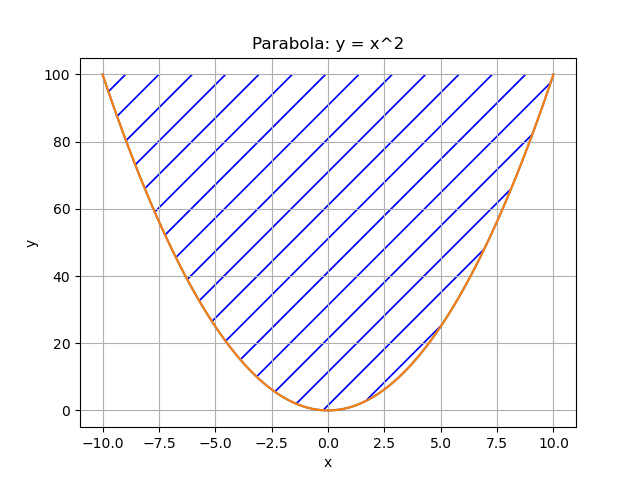
\includegraphics[width=0.4\textwidth]{img/parabola.png}
\end{center}

\es the line
\ei the filled area
\ei red dots
\ei square of blue dots, including the diagonal
\ei The representation of a reflexivity relation in rational numbers is the diagonal line on a 2D
    plane. The representation of a symmetry of a set on a 2D plane is the set itself and its mirror
    image across the diagonal
\ei TODO: Something like this?
    \begin{center}
    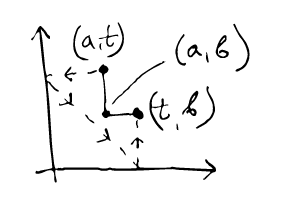
\includegraphics[width=0.3\textwidth]{img/heuristic.png}
    \end{center}
\ee

\exercise{2.6.1.10}

Consider the binary relation $R = \set{(n,n+1)|n\in\Z}\subseteq\Z\times\Z$.

\es What is the equivalence relation generated by $R$?
\ei How many equivalence classes are there?
\ee

\ans

\es Whole $\Z$.
\ei One.
\ee

\exercise{2.6.1.11}

Suppose $N$ is a network (or graph). Let $X$ be the nodes of the network, and
let $R \subseteq X \times X$ denote the relation such that $(x, y) \in R$ iff
there exists an arrow connecting $x$ to $y$.

\es What is the equivalence relation $\sim$ generated by $R$?
\ei What is the quotient $X/\sim$?
\ee

\ans

\es For each disjoint subgraph $g \subseteq N$, the relation $R$ represents a
    fully connected graph $g'$ formed by the vertices of $g$.
\ei A set of disjoint graphs.
\ee

\exercise{2.6.2.4}

(The picture) Write down the cardinality of $P \cong \underline{n}$ as a natural
number $n \in \N$.

\ans

$1$, because the described $W \to X$ and $W \to Y$ make all elements of $X$ and
$Y$ equivalent.

\exercise{2.6.2.5}

Suppose that $W = \emptyset$; what can you say about $X \sqcup_W Z$?

\ans

$X \sqcup_W Z$ becomes $X \sqcup Z$ because $(X \sqcup W \sqcup Z)/\sim$ is
filled with distinct elements of both $X$ and $Z$.

\exercise{2.6.2.6}

Let $W := \N = \set{0,1,2,... }$ denote the set of natural numbers, let $X =
\mathbb{Z}$ denote the set of integers, and let $Y = \set{\Smiley}$ denote a
one-element set. Define $f : W \to X$ by $f(w) = -(w+1)$, and define $g: W \to Y$ to be
the unique map. Describe the set $X \sqcup_W Y$ .

\ans

$X \sqcup_W Y = \set{\Laughey, 1, 2, 3}$ where $\Laughey$ is equivalent to all
the items of $\set{..., -2, -1, 0, \Laughey}$.

\exercise{2.6.2.7}

Let $i: R \subseteq X \times X$ be an equivalence relation. Composing with the
projections $\pi_1, \pi_2 : X \times X \to X$, we have two maps $\pi_1 \circ i :
R \to X$ and $\pi_2 \circ i: R \to X$.

\es What is the pushout $X - R - X$
\ei If $i: R \subseteq X \times X$ is not assumed to be an equivalence relation,
    we can still define the pushout above. Is there a relationship between the
    pushout $X - R - X$ and the equivalence relation generated by $R \subseteq X
    \times X$
\ee

\ans

\es For any equivalence class in $R$, the pushout $X \sqcup_{i} X$ merges all
    the points belonging to it into a single element.
\ei If $i' : R' \subseteq X \times X$ is not an equivalence relation, then its
    pushout $|X \sqcup_{i'} X| > |R|$ where $R$ is the equivalence relation
    generated by $R'$.
\ee

\exercise{2.6.3.2}

Let $X = R$ be the set of real numbers. What is the coequalizer of the two maps
$X \to X$ given by $f = x \mapsto x$ and $g = x \mapsto (x + 1)$ respectively?

\ans

The coequalizer $Coeq(f,g) \sim [0,1) \subset \Rat$.

\exercise{2.6.3.3}

Find a universal property enjoyed by the coequalizer of two arrows.

\ans

For any set $A$, function $f$ and $g$, there exists unique $u$ mapping
$Coeq(f,g)$ to $A$ such that everything commute, in particular, $u \circ i = q$.

\begin{center}
% https://tikzcd.yichuanshen.de/#N4Igdg9gJgpgziAXAbVABwnAlgFyxMJZABgBoBmAXVJADcBDAGwFcYkQBhCGARwAoAZqQDmAShABfUuky58hFGQBM1Ok1bsAgpOkgM2PASJkAjKoYs2iEAE0dMg-OOli59VZAANSaphRh8ESgAgBOEAC2SGQgOBBIJjSMWGAeUPRwABZ+9iChEUjkNLFISonJqRDMAEaMbDRZ9FBIYMyMjEX0WIzskCk5eZGIpTFxiCZSwWGDw8WI0VUwYE2IAGwA7BKUEkA
\begin{tikzcd}
X \arrow[d, Rightarrow, "g", "f"']             \\
Y \arrow[d, "q"] \arrow[dd, bend left=67, "i"] \\
A                                              \\
{Coeq(f,g)} \arrow[u, dashed, "\exists!u"]
\end{tikzcd}
\end{center}


\exercise{2.6.3.4}

(Initial object). An initial set is a set S such that for every set A, there
exists a unique function $S \to A$

\es Find an initial set
\ei Do you think that the notion initial set belongs in this section (Section
    2.6)? How so? If coproducts, pushouts, and coequalizers are all colimits,
    what do colimits have in common?
\ee

\ans

\es Initial object for sets is the empty set.
\ei Colimits are isomorphic up to the unique isomorphism (???)
\ee

\subsection{Other notions in Set}

\exercise{2.7.1.2}

Create an olog that includes sets $X$ and $Y$ , and functions $f : X \to Y$ and
$g: Y \to X$ such that $g \circ f = id_X$ but such that $f \circ g \ne id_Y$;
that is, such that $f$ is a retract section but not an isomorphism.

\ans

Any $X$ and $Y$ meet this condition if $|X| < |Y|$. For example, mothers and
their children. We may say that $f:X \to Y$ maps mothers to their first
children, while $g:Y \to X$ maps children to their mothers.

\exercise{2.7.2.2}

For a finite set $A$, let $|A| \in \N$ denote the cardinality of (number of
elements in) $A$. If $A$ and $B$ are both finite (including the possibility that
one or both are empty), is it always true that $|B^A| = |B|^{|A|}$?

\ans

The statement is true when both sets are non-empty and if only one set is empty.
When both sets are empty, it is true if we put $0^0 = 1$.

\exercise{2.7.2.4}

Let $X = \set{1, 2}$, $A = \set{a, b}$, and $Y = \set{x, y}$

\es Write down three distinct elements of $L := Hom_{Set}(X \times A, Y)$
\ei Write down all the elements of $M := Hom_{Set}(A, Y)$
\ei For each of the three elements $l \in L$ you chose in part (a), write down
    the corresponding function $\phi(l): X \to M$ guaranteed by Proposition
    2.7.2.3.
\ee

\ans

\es E.g.
    $l_1 = \set{(1,a) \mapsto x, (1,b) \mapsto x, (2,a) \mapsto x, (2,b) \mapsto x}$,
    $l_2 = \set{(1,a) \mapsto x, (1,b) \mapsto x, (2,a) \mapsto x, (2,b) \mapsto y}$,
    $l_3 = \set{(1,a) \mapsto x, (1,b) \mapsto x, (2,a) \mapsto y, (2,b) \mapsto x}$
\ei There are:
    $f_{xx} = \set{a \mapsto x, b \mapsto x}$,
    $f_{xy} = \set{a \mapsto x, b \mapsto y}$,
    $f_{yx} = \set{a \mapsto y, b \mapsto x}$,
    $f_{yy} = \set{a \mapsto x, b \mapsto y}$
\ei $\phi(l_1) = \set{1 \mapsto f_{xx}, 2 \mapsto f_{xx}}$,
    $\phi(l_2) = \set{1 \mapsto f_{xx}, 2 \mapsto f_{xy}}$,
    $\phi(l_3) = \set{1 \mapsto f_{xx}, 2 \mapsto f_{yx}}$
\ee

\exercise{2.7.2.5}

Let $A$ and $B$ be sets.  We know that $Hom_{Set}(A, B) = B^A$, so we have a
function $id_{B^A} : Hom_{Set}(A, B) \to B^A$. Look at Proposition 2.7.2.3,
making the substitutions $X = Hom_{Set}(A, B)$, $Y = B$, and $A = A$. Consider
the function

\vsp

$\phi^{-1} : Hom{Set}(Hom_{Set}(A, B), B^A) \to Hom_{Set}(Hom_{Set}(A, B) \times A, B)$

\vsp

obtained as the inverse of (2.42).  We have a canonical element $id_{B^A}$ in
the domain of $\phi^{-1}$.  We can apply the function $\phi^{-1}$ and obtain an
element $ev = \phi^{-1}(id_{B^A}) \in Hom_{Set}(Hom_{Set}(A, B) \times A, B)$,
which is itself a function:

\vsp
$ev: Hom_{Set}(A, B) \times A \to B$
\vsp

\es Describe the function $ev$ in terms of how it operates on elements in its domain.
\ei Why might one be tempted to denote this function by $ev$?
\ee

\ans

\es According to (2.4),
$\phi^{-1}$ is
\[
\psi : [(A \to B) \to (A \to B)] \to [(A \to B) \times A \to B]
\]
defined as
\[
\psi = (g:G) \mapsto ((f, a): (A \to B)\times A) \mapsto g(f)(a)
\]
where we put $G = [(A \to B) \to (A \to B)]$. Indeed, $G$ has an identity
element $id_{B^A} = f \mapsto f$.
Now, \[ev = \psi(id_{B^A}) = (f,a) \mapsto id_{B^A}(f)(a) = (f,a) \mapsto b\]
where $f: A \to B = a \mapsto b$

\ei $ev$ must be a shortening of "evaluate". It maps $f$ and its input argument
    to the result.

\ee

\exercise{2.7.2.6}

In Example 2.4.1.7 we said that $\Rational^2$ is an abbreviation for $\Rational
\times \Rational$, but in (2.43) we say that $\Rational^2$ is an abbreviation
for $\Rational^{\underline{2}}$. Use Exercise 2.1.2.14, Proposition 2.7.2.3,
Exercise 2.4.2.10, and the fact that $1+1=2$, to prove that these are
isomorphic, $\Rational^{\underline{2}} = \Rational \times \Rational$

\ans

Reminder:

2.1.2.14: Find a set A such that for any set X there is a isomorphism of sets $X
= Hom_{Set}(A,X)$ (Answer - $\set{\Smiley}$).

2.7.2.3: Currying

2.4.2.10: Universal property of coproducts: $Hom_{Set}(X,A) \times
Hom_{Set}(Y,A) = Hom_{Set}(X \sqcup Y, A)$.


So we go:

\[
\Rat^{\underline 2} = \set{1,2} \to \Rat \cong \set{1} \sqcup \set{2} \to
\Rat \cong (\set{1} \to \Rat) \times (\set{2} \to \Rat) \cong \Rat \times \Rat
\]

where we write $Hom_{Set}(A,B)$ as just $A \to B$.

\unsure The problem in the proof is that we didn't use currying and the $1+1=2$
fact. Should we actually continue by saying that $\Rat \times \Rat =
\Rat^{1+1}$? But then again, what about currying?

\exercise{2.7.3.2}

Everything in Proposition 2.7.3.1 is true except in one case, namely
that of
\[
  \underline{0}^{\underline{0}}
\]

In this case, we get conflicting answers, because for any set A, including $A =
\emptyset = \underline{0}$, we have claimed both that $A^0 = \underline{1}$ and
that $0^A = \underline{0}$.  What is the correct answer for
$\underline{0}^{\underline{0}}$, based on the definitions of $\underline{0}$ and
$\underline{1}$, given in (2.6), and of $A^B$, given in (2.41)?

\ans

Reminder:

2.41: $B^A := Hom_{Set}(A,B)$, which we sometimes write just as $A \to B$.

2.6: The definitions are: $\underline{1} := \set{1}$, $\underline{0} := \emptyset$.

\vsp

$Hom_{Set}(A,B)$, by definition, consists of sets of the form
$\set{(a_1,b_1),(a_2,b_2),...}$ where $\set{a_1, a_2, ...} = A$ and $\forall i:
b_i \in B$.  In contrast to $Hom_{Set}(A,\set{})$, for which we can not define
any such functions, in $Hom_{Set}(\set{}, \set{})$ we can define a single empty
function, so $Hom_{Set}(\set{}, \set{}) = \set{\set{}}$. Thus:

\[
  \underline{0}^{\underline{0}} \cong \underline{1}
\]

\exercise{2.7.3.3}

It is also true of natural numbers that if $a, b \in \N$ and $ab = 0$ then either
$a = 0$ or $b = 0$. Is the analogous statement true of all sets?

\ans

The proposition is: if $A \times B = \set{}$ then either $A = \set{}$ or $B = \set{}$.

TODO: check the proof of this fact for numbers.

\exercise{2.7.3.4}

Explain why there is a canonical function $\U{5}^\U{3} \times \U{3} \to \U{5}$ but not a
canonical function $\U{575} \to \U{5}$.

\ans

Following the definition of Currying (2.7.2.3), we can transform $\U{5}^\U{3}
\times \U{3} \to \U{5}$ back to $Hom_{Set}(\U{3},\U{5}) \to
Hom_{Set}(\U{3},\U{5})$.  There is an canonical function
$id_{Hom_{Set}(\U{3},\U{5})}$ mapping every $\U{3} \to \U{5}$ function to
itself.

In contrast, for $\U{575} \to \U{5}$ which is $Hom_{Set}(\U{575},\U{5})$ we
can't name any outstanding functions.

\exercise{2.7.4.2}

\es How many elements does $\Pow(\emptyset)$ have?
\ei How many elements does $\Pow(\set{\Smiley})$ have?
\ei How many elements does $\Pow(\set{1, 2, 3, 4, 5, 6})$ have?
\ei Any idea why they may have named it "power set"?
\ee

\ans

\es $\Pow(\emptyset) = \set{\emptyset}$ - one element.
\ei $\Pow(\set{\Smiley}) = \set{\set{}, \set{\Smiley}}$ - two elements.
\ei $\Pow(\set{1, 2, 3, 4, 5, 6})$ has $64$ elements.
\ei The name probably originates from the fact that $|\Pow(A)| = 2^{|A|}$.
\ee

% \example{2.7.4.5}
% Let $n \in \N$ be a natural number and let $V = \U{n + 1}$. Define the
% n-simplex, denoted $\Delta^n$, to be the simplicial complex $\Pow(V) \subseteq
% \Pow(V)$, i.e. the whole power set, which indeed is downward-closed and contains
% all atoms

\exercise{2.7.4.6}

Let $X$ be the following simplicial complex, so that $X_0 = \set{A, B, ... , M}$

\begin{center}
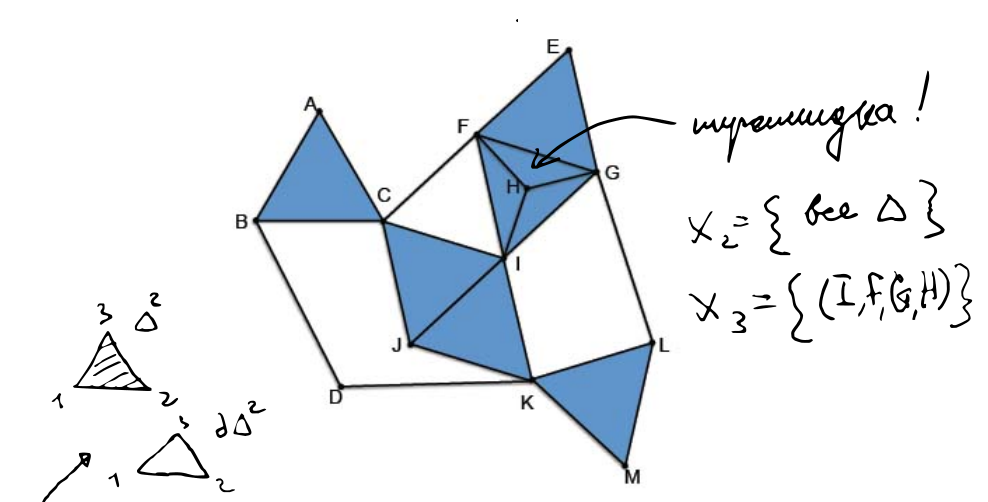
\includegraphics[width=0.8\textwidth]{img/simplicial_complex.png}
\end{center}

TODO: insert a clean picture

In this case $X_1$ consists of elements like $\set{A,B}$ and $\set{D,K}$ but not
$\set{D,J}$.  Write out $X_2$ and $X_3$ (hint: the drawing of $X$ indicates that
$X_3$ should have one element).

\ans

$X_2 = \set{ABC, CIJ, IJK, KLM, EFG, FGH, GHI, FHI, IFG}$ (all the blue
trinagles).

$X_3 = \set{IHGF}$ (the pyramid).

\exercise{2.7.4.7}

The 2-simplex $\Delta^2$ is drawn as a filled-in triangle with vertices $V =
\set{1, 2, 3}$. There is a simplicial complex $X = \delta \Delta^2$ that would
be drawn as an empty triangle with the same set of vertices.

\es Draw $\Delta^2$ and $X$ side by side and make clear the difference.
\ei Write down the data for X as a simplicial complex. In other words what are
    the sets $\set{X_0, X_1, X_2, X_3, ...}$?
\ee

\ans
\begin{center}
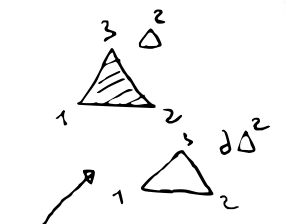
\includegraphics[width=0.2\textwidth]{img/simplicial_complex_example.png}
\end{center}
\es (TODO: insert a clean picture).
\ei $X_0 = \set{1,2,3}$, $X_1 = \set{(1,2), (1,3), (2,3)}$, $X_2 = X_3 = ... =
    \emptyset$.
\ee

\exercise{2.7.4.12}

Let $f: A \to \Omega$ denote the characteristic function of some $A' \subseteq A$, and
define $A'' \subseteq A$ to be its complement, $A'' = A - A'$ (i.e. $a \in A''$
if and only if $a \notin A'$).

\es What is the characteristic function of $A'' \subseteq A$?
\ei Can you phrase it in terms of some function $\Omega \to \Omega$?
\ee

\ans

$g: A'' \to \Omega = not \circ f$

where

$not: \Omega \to \Omega = \set{True \mapsto False, False \mapsto True}$.

\exercise{2.7.5.6}

Show, in analogy to Proposition 2.7.5.5, that pushouts preserve epimorphisms.

\ans

Let $f: Y \to X$ be an epimorphism. For any function $g$, the bottom map $f':A
\to X \sqcup_Y A$ is again an epimorphism.

\begin{center}
% https://tikzcd.yichuanshen.de/#N4Igdg9gJgpgziAXAbVABwnAlgFyxMJZABgBpiBdUkANwEMAbAVxiRAE0QBfU9TXfIRQBGclVqMWbABrdeIDNjwEiZYePrNWiEAEE5fJYKKj11TVJ3SABAB1bcAI4BjJmgD67a-p6GBKlAAmUkCNSW0QACFucRgoAHN4IlAAMwAnCABbJDIQHAgkUQktNhSDEHSsnOp8pGDiyxB7FIg0xgZrePLK7MR62sQAZnNw0oBybozeooHhhoj4id8KqaQ5gYAWagYsMAioCCYAIwZWagALGDooJDAmBgYauiwGNkg9kBGSnWzlnsKagVEFsQDsPjoDsdTp8QJdrrd7o88s9Xjp3mcQEcYGAbkNchYIo5JlU+oCkCCsTikABaQb40Y6NAxLhAA
\begin{tikzcd}
Y \arrow[r, "f"] \arrow[d, "\forall g"]        & X \arrow[d, "g'"] \arrow[rdd, "r", "q"', Rightarrow, bend left] &   \\
A \arrow[r, "f'"] \arrow[rrd, "p", bend right] & X \sqcup_Y A \arrow[rd, "n", "m"', Rightarrow]                  &   \\
                                               &                                                           & B
\end{tikzcd}
\end{center}

The proof goes as follows:
(1) We add some $B$ and two functions $m,n: X \sqcup_Y A \to B$ such that $m
\circ f' = n \circ f'$. We denote this function by $p$. (2) We look at the
functions $q = m \circ g'$ and $r = n \circ g'$: $q \circ f = m \circ g' \circ f
= m \circ f' \circ g = n \circ f' \circ g = n \circ g' \circ f = r \circ f$. So
we can speak of only one function $q$ and ignore $r$. (3) From the universal
property of pushouts, there exist exactly one function $X \sqcup_Y A \to B$, so
we have $m = n$. (4) We conclude that $f'$ is an epimorphism by the definition.


\exercise{2.7.5.9}

Consider the subobject classifier $\Omega$, the singleton $\set{\Smiley}$ and
the map $\set{\Smiley} \to_{True} \Omega$ from Definition 2.7.4.9. Look at
diagram 2.44 (below) and in the spirit of Exercise(sic!) 2.7.5.7, come up with a
label for $\Omega$, a label for $\set{\Smiley}$, and a label for $True$. Given a
label for $X$ and a label for $f$, come up with a label for $A$, a label for $i$
and a label for $f'$, such that the English smoothly fits the mathematics.


\begin{center}
% https://tikzcd.yichuanshen.de/#N4Igdg9gJgpgziAXAbVABwnAlgFyxMJZABgBpiBdUkANwEMAbAVxiRAEEQBfU9TXfIRQBGclVqMWbAMoBbLA268QGbHgJEyw8fWatEIABpK+awUVHbquqQYA6dgPKyYAczrdxMKK-hFQAGYAThCySGQgOBBIohJ6bAEA5CYgwaHh1FFIAEzWkvogWClpYYi5kdGIAMx58QYBxSGlsVnVtbYgACpBUlwUXEA
\begin{tikzcd}
A \arrow[r, "f'"] \arrow[d, "i"] & \{ \Smiley \} \arrow[d, "True"] \\
X \arrow[r, "f"]                 & \Omega
\end{tikzcd}
\end{center}

\ans


\begin{center}
% https://tikzcd.yichuanshen.de/#N4Igdg9gJgpgziAXAbVABwnAlgFyxMJZABgBpiBdUkANwEMAbAVxiRAEEQBfU9TXfIRQBGclVqMWbAMoBbLA268QGbHgJEyw8fWatEIABpK+awUVHbquqQYA6dgPKyYAczrdxMKK-hFQAGYAThCySGQgOBBIohJ6bAEA5CYgwaHh1FFIAEzWkvogWClpYYi5kdGIAMx58QYBxSGlsVnVtbYgACpBUlwUXEA
\begin{tikzcd}
\fbox{X which matches a Pattern} \arrow[rr, "matches"] \arrow[d, "is"] & & \fbox{Pattern} \arrow[d, "is"] \\
\fbox{X} \arrow[rr, "matches"]                 & & \fbox{Example}
\end{tikzcd}
\end{center}

\exercise{2.7.6.2}

\es Come up with some notion of mapping for multisets that generalizes functions
    when the notion is restricted to sets.
\ei Suppose that $X = (1, 1, 2, 3)$ and $Y = (a, b, b, b)$, i.e. $X = \{1, 2,
    3\}$ with $1$ having multiplicity $2$, and $Y = \{a, b\}$ with $b$ having
    multiplicity $3$. What are all the maps $X \to Y$ in your notion?
\ee

\ans

\es The right definition is given in the textbook below this exercise. Here we
    try a brute-force approach. Let Multiset be a set of pairs $\{(e_i,n_i)\}$
    where $\set{e_i} = E$ is the set of elements and $n_i \in \N : n_i \ge 1$
    the multiplicity of each element.

    With this definition, $X = \set{(1,2),(2,1),(3,1)}$ and $Y = \set{(a,1),
    (b,3)}$.
\ei We are going to have some troubles with the definition of what the map is in
    our multiset. We want to preserve the totality, so we define map $A \to B$
    as a set of pairs $\set{((a_i, n_i), B_i)}$ where $B_i \subseteq B$ such that
    (1) every $(a_i,n_i)$ is unique among the map, (2) $\set{(a_i,n_i)} = A$,
    (3) sum of multiplicities of $B_i$ is equal to the $n_i$.

    Some examples of $X \to Y$ are:
    \es $\set{((1,2),\set{(a,1),(b,1)}),((2,1),\set{(a,1)}),((3,1),\set{(a,1)})}$
    \ei $\set{((1,2),\set{(b,2)}),((2,1),\set{(a,1)}),((3,1),\set{(a,1)})}$
    \ei $\set{((1,2),\set{(b,2)}),((2,1),\set{(b,1)}),((3,1),\set{(b,1)})}$
    \ei ...
    \ee

    TODO: should we really list all the maps?
\ee

\exercise{2.7.6.4}

Suppose that a pseudo-multiset is defined to be almost the same as a multiset,
except that $\pi$ is not required to be surjective.

\es Write down a pseudo-multiset that is not a multi-set.
\ei Describe the difference between the two notions in terms of multiplicities.
\ei The multiset commutative diagram might no longer commute for the
    pseudo-multisets.
\ee

\ans

Recap: We say that $f: X \to Y$ is surjective if, for all $y \in Y$ there exists
some $x \in X$ such that $f(x) = y$. In other words, uncovered elements in $Y$
are not allowed, but $X$ can be larger than $Y$.  Being "non-surjective" means
that the multiset is allowed to contain unused names in it.

\es Example of a pseudo-multiset which is not a multiset: $(E =
    \set{1_1,1_2,2,3}, B = \set{1, 2, 3, \Smiley}, \pi = \set{1_1 \mapsto 1, 1_2
    \mapsto 1, 2 \mapsto 2, 3 \mapsto 3})$. $\pi$ doesn't map anything to
    \Smiley thus it is not surjective.
\ei Pseudo-multisets are allowed to contain elements with undefined
    multiplicities.
\ei Pseudo-multisets are less useful because it is hard to choose what is
    better: to include an element with an undefined multiplicity or to not
    include it at all.
\ee

\exercise{2.7.6.5}

Consider the multisets described in Exercise 2.7.6.2.

\es Write each of them in the form $(E, B, \pi)$, as in Definition 2.7.6.3.
\ei In terms of the same definition, what are the mappings $X \to Y$ ?
\ei If we remove the restriction that diagram 2.45 must commute, how many
    mappings $X \to Y$ are there?
\ee

\ans

\es $X = (E =
    \set{1_1,1_2,2,3}, B = \set{1, 2, 3}, \pi = \set{1_1 \mapsto 1, 1_2
    \mapsto 1, 2 \mapsto 2, 3 \mapsto 3})$.

    $Y = (E = \set{a, b_1, b_2, b_3}, B = \set{a,b}, \pi = \set{a \mapsto a, b_1
    \mapsto b, b_2 \mapsto b, b_3 \mapsto b})$.
\ei The set of mappings is $\set{(f_1, f_2) | f_2(\pi_X(x)) =
    \pi_Y(f_1(x))}$. It is the set containing all $f_1: E_X \to E_Y$ except
    those which leads to different instances of $B_X$ to have different names in
    $B_Y$. So, for example, $\set{1_1 \mapsto a, 1_2 \mapsto b_1}$ is forbidden.
\ei Without the commutativity restriction, we must have $|E_X \to E_Y| * |B_X
    \to B_Y| = 4^4 * 3^2 = 2304$ different mappings.
\ee

\exercise{2.7.6.8}

Given sets $X$, $Y$, $Z$ and functions $f : X \to Y$ and $g: Y \to Z$, we can
compose them to get a function $X \to Z$. If $B$ is a set, if $(X, p)$, $(Y,
q)$ and $(Z, r)$ are relative sets over $B$, and if $f : (X, p) \to (Y, q)$ and
$g: (Y, q) \to (Z, r)$ are mappings, is there a reasonable notion of composition
such that we get a mapping of relative sets $(X, p) \to (Z, r)$? Hint: draw
diagrams.

\ans

\begin{center}
% https://tikzcd.yichuanshen.de/#N4Igdg9gJgpgziAXAbVABwnAlgFyxMJZABgBpiBdUkANwEMAbAVxiRAA0QBfU9TXfIRQBGclVqMWbAJrdeIDNjwEiAJlLDx9Zq0QgAWnL5LBRMqq2TdIAELdxMKAHN4RUADMAThAC2SMiA4EEiiEjps7kYgXr4h1EFI6mFSek5RMX6IAQmISdopIAAW6d6Z2cGIAMzUDHQARjAMAAr8ykIgDDDuOCDU+dZoJbG58RXVydaeQ5mhOeP9bACO9lxAA
\begin{tikzcd}
X \arrow[r, "f"] \arrow[rrd, "h"] \arrow[dd, "p"] & Y \arrow[rd, "g"] \arrow[ldd, "q"] &                    \\
                                                  &                                    & Z \arrow[lld, "r"] \\
B                                                 &                                    &
\end{tikzcd}
\end{center}

We can define $h : X \to Z = g \circ f$ and the since all the $p,q,r$ triangles
do commute by the definition of mappings of relative sets. So if we have
$f_{rel} : (X,p) \to (Y,q)$ and $g_{rel} : (Y,q) \to (Z,r)$ then $g_{rel} \circ
f_{rel}$ is just $g \circ f$.

\exercise{2.7.6.9}

\es Let $\set{\Smiley}$ denote a set with one element. What is the difference
    between sets over $\set{\Smiley}$ and simply sets?
\ei Describe the sets relative to $\emptyset$. How many are there?
\ee

\ans

\es We need to explore the $Hom_{RelSet}((A,a),(B,b))$ where both $A$ and $B$
    are relative to $E=\set{\Smiley}$ and $a,b$ are unique mappings from $A,B$
    to $E$.
    \begin{itemize}
    \item $A$ and $B$ are non-empty: trivial. The behaviour is similar to
          $Hom_{Set}(A,B)$.
    \item $A$ is empty: The only possible $a:A \to E$ is $\set{}$. The problem
          might come from the fact that $a$ must be a part of commutative
          triangle with $b$. TODO: check if we can say that empty function
          commutes with anything or not.
    \item $B$ is empty: The only possible $f:A \to B$ is $\set{}$ when $A$ is
          also empty. Again, need to check the triangle commutement statement
          for empty functions.
    \end{itemize}
\ei In order for $(S,\pi)$ to be relative to $\set{}$, the $\pi:S \to \set{}$
    must exist which is possible only if $S$ is also empty. Thus, we have only
    one set relative to the empty set.
\ee

\exercise{2.7.6.13}

Let $\set{\Smiley}$ denote a one element set. What are $\set{\Smiley}$-indexed
sets and mappings between them?

\ans

The $\set{\Smiley}$-indexed sets are equivalent to just sets and the mappings
between them are equivalent to functions over sets.

\exercise{2.7.6.14}

There is a strong relationship between $A$-indexed sets and relative sets over
$A$. What is it?

\ans

For any  $I$-relative set $A_I$, where $I$ is also an index set of some
$(S_a)_{a\in I}$, $A_I$ could be used as an alternative index set. TODO: not
sure.

\section{Categories and functors, without admitting it}

\subsection{Monoids}

\exercise{3.1.1.6}

Let $M = \N$ be the set of natural numbers. Taking $e = 1$, come up with a
formula for $*$ that gives $\N$ the structure of a monoid.

\ans

We set $*$ is multiplication. Then we have both identitites $a*e = a$, $e*a = a$
and the associativity.


\exercise{3.1.1.7}

Come up with an operation on the set $M = \set{1, 2, 3, 4}$, i.e. a legitimate
function $f : M \times M \to M$, such that $f$ cannot be the multiplication
formula for a monoid on $M$. That is, either it is not associative, or no
element of $M$ can serve as a unit.

\ans

\es Has unit, but is not associative: $f = (a,b) \mapsto max(div(a,b), 1)$
    modulo $4$, where $div$ denotes integer division.
\ei Associative, but has no unit: any function returning a constant element, say
    $1$.
\ee

\exercise{3.1.1.8}

In both Example 3.1.1.3 and Exercise 3.1.1.6, the monoids $(M, e, *)$ satisfied
an additional rule called commutativity, namely $m*n = n*m$ for every $m$, $n
\in M$.  There is a monoid $(M, e, *)$ lurking in linear algebra textbooks that
is not commutative; if you have background in linear algebra try to answer this:
what $M$, $e$, and $*$ might I be referring to?

\ans

$M = \set{1,a,b}$ \href{https://math.stackexchange.com/a/207813/374432}{link}.

\exercise{3.1.1.9}

Recall the notion of commutativity for monoids from Exercise 3.1.1.8.

\es What is the smallest set $M$ that you can give the structure of a
    non-commutative monoid?
\ei What is the smallest set $M$ that you can give the structure of a monoid?
\ee

\ans

\es Three-element set. It will not work for two-element set $\set{a,b}$ because
    the non-associativity condition $a*b \ne b*a$ is not compatible with the
    monoid identity laws.
\ei One-element set is the smallest set which can have a monoid structure, its
    only element must be the monoid's identity.
\ee

\exercise{3.1.1.16}

Let $\set{\Smiley}$ denote a one-element set.

\es What is the free monoid generated by $\set{\Smiley}$?
\ei What is the free monoid generated by $\emptyset$?
\ee

\ans

\es The $\set{\Smiley}$ generates the monoid $(M,[],++)$ where $M$ is the set of
    lists \[\set{(0,\set{}), ..., (n,\set{i \mapsto \Smiley | i \in {1..n}}),
    ...}\] In other words, it is a set of all possible lists of $\Smiley$ of
    different lengths.
\ei $\emptyset$ generates a monoid consisting of the empty list alone:
    $(\set{[]}, [], ++)$.
\ee

\exercise{3.1.1.21}

Let's consider the buffer concept again (see Application 3.1.1.20), but this
time only having size 3 rather than size 32. Show using Definition 3.1.1.17 that
with relations given by $\sim_1$ we indeed have $[a, b, c, d, e, f] = [a, b, f]$
and that with relations given by $\sim_2$ we indeed have $[a, b, c, d, e, f] =
[a, b, c]$.

\ans

We can to state that in order to use $\sim_1$ and $\sim_2$ we need to extend the
task by defining buffers of size 4 and 5. The answer seems obvious assuming that
we accept this assumption.

TODO

\exercise{3.1.1.22}

Let $K := \set{BS, a, b, c, ... , z}$ a set having 27 elements. Suppose you want
to think of $BS \in K$ as the “backspace key” and the elements $\set{a, b, ...
z} \in K$ as the letter keys on a keyboard. Then the free monoid $List(K)$ is
not quite appropriate as a model because we want $[a, b, d, BS] = [a, b]$.

\es Choose a set of relations for which the monoid presented by generators $K$
    and the chosen relations is appropriate to this application.
\ei Under your relations, how does $[BS]$ compare with $[]$? Is that suitable?
\ee

\ans


\es The set of relations is $\set{[i,BS] \sim [] | i \in \set{a,..., z}}$.
\ei Adding $[BS]$ makes list smaller rather than larger. With respect to the
    relations, we can say that $[BS]$ has negative length.
\ee

\exercise{3.1.1.27}

(Classify the cyclic monoids). Classify all the cyclic monoids up to
isomorphism. That is, come up with a naming system such that every cyclic monoid
can be given a name in your system, such that no two non-isomorphic cyclic
monoids have the same name, and such that no name exists in the system unless it
refers to a cyclic monoid.

Hint: one might see a pattern in which the three monoids in Example 3.1.1.25
correspond respectively to $\infty$, $1$, and $12$, and then think "Cyclic
monoids can be classified by (i.e. systematically named by elements of) the set
$\N \cup \set{\infty}$". That idea is on the right track, but is not correct.

\ans

Since the cyclic monoids are built on just one generator, it does not matter how
many relationships we define for it. Only the relationship with the smallest
maximum argument is important, e.g. $[Q,Q],[Q,Q,Q]$ is more important then
$[Q],[Q,Q,Q,Q]$.

So, any cyclic monoid can be classified by two numbers: the length of
"tail" and the length of "loop".

\exercise{3.1.2.4}

\es Realize the set $T := [0,12) \subseteq \Rat$ as the coequalizer of a pair of
    arrows $\Rat \toto \Rat$.
\ei For any $x \in \Rat$, realize the mapping $x \cdot-: T \to T$, implied by
    Example 3.1.2.3, using the universal property of coequalizers.
\ei Prove that it is an action.
\ee

\ans

Note: $T = \set{x \in \Rat | 0 \leq x < 12}$.

Note: The coequalizer of $f$ and $g$ is $Coeq(f,g) := Y / f(x) \sim g(x)$ i.e.
the coequalizer of f and g is the quotient of Y by the equivalence relation
generated by $\set{(f(x),g(x)) | x \in X} \subseteq Y \times Y$

\es Indeed, consider an identity $f:\Rat \to \Rat = x \mapsto x$ and $g:\Rat \to
    \Rat = x \mapsto x + 12$. Their coequalizer is in 1-1 correspondence with
    the $[0,12)$ range on $\Rat$.
\ei Consider the diagram for coequalizer universal property. Assume that there
    exists $q : \Rat \to (\Rat \to T)$ such that $q \circ f = q \circ g$.
    \begin{center}
    \begin{tikzcd}
    \Rat \arrow[d, Rightarrow, "g", "f"']             \\
    \Rat \arrow[d, "q"] \arrow[dd, bend left=67, "i"] \\
    (\Rat \to T)                                      \\
    {T:=Coeq(f,g)} \arrow[u, dashed, "\exists!u"]
    \end{tikzcd}
    \end{center}
    The universal property of coequalizer states that there exists a unique $u:
    T \to (\Rat \to T)$ where $T = Coeq(f,g)$. Now we can define $u = t \mapsto r
    \mapsto (t + r) `mod` 12$.

\ei (1) $t \mapsto 0 \mapsto (t `div` 12 = t)$. (2) $t \mapsto (a + b) \mapsto
    (t + a + b)`div` 12 = (((t + a)`div` 12) + b) `div` 12$.
\ee

\exercise{3.1.2.5}

Let $B$ denote the set of buttons (or positions) of a video game controller
(other than, say 'start' and 'select'), and consider the free monoid $List(B)$
on $B$.

\es What would it mean for $List(B)$ to act on the set of states of some game?
    Imagine a video game $G'$ that uses the controller, but for which $List(B)$
    would not be said to act on the states of $G'$ . Now imagine a simple game
    $G$ for which $List(B)$ would be said to act.
\ei Can you think of a state $s$ of $G$, and two distinct elements $l, l' \in
    List(B)$ such that $l \circlearrowright s = l' \circlearrowright s$?  In
    video game parlance, what would you call an element $b \in B$ such that, for
    every state $s \in G$, one has $b \circlearrowright s = s$?
\ei In video game parlance, what would you call a state $s \in S$ such that, for
    every sequence of buttons $l \in List(B)$, one has $l \circlearrowright s =
    s$?
\ee


\ans

\es The $G$ could be a simple maze game. Can $G'$ be a non-deterministic game,
    where state changes happen as a result of both user actions $List(B)$ and
    the outcome of some random number generator?
\ei (1) For maze game: the maze with more than one solution. (2) An unused
    button.
\ei A terminal state? A hunged (buggy) game?
\ee

\exercise{3.1.2.13}

Notes: Let $A = Hom_{Set}(List(\sum) \times S, S)$ and $B = Hom_{Set}(\sum
\times S, S)$, let $\phi: A \to B$ and $\psi: B \to A$, also let $f \in A$ and
$g \in B$.
\vsp
Consider the functions $\phi$ and $\psi$ defined above.
\es Show that for any $g : \sum \times S \to S$, the map $\psi(g) : List(\sum)
    \times S \to S$ constitutes an action.
\ei Show that $\phi$ and $\psi$ are mutually inverse functions (i.e. $\phi \circ \psi =
    id_{Hom(\sum \times S,S)}$ and $\psi \circ \phi = id_{A}$)
\ee

\ans

\es $\forall g, \psi(g) = (l,s) \mapsto \psi(g)(l_{0..-1}, g(l_{-1},s))$ with a
    special case of $\psi(g) = ([],s) \mapsto s$. Now, $\psi(g)$ is an
    action, because: (1) $\psi(g)([],s) \mapsto s$ by definition; (2)
    $\psi(g)(l + l') = g(l_0, ... g(l'_{-2}, g(l'_{-1}, s))) = \psi(g)(l,
    \psi(g)(l', s))$
\ei (1) $\phi(\psi(g)) = (\epsilon, s) \mapsto \psi(g)([\epsilon], s) = g(\epsilon, s)$
    (2) $\psi(\phi(f)) = (l,s) \mapsto \psi(\phi(f))(l_{0..-1}, \phi(f)(l_{-1},
    s)) = f([l_0], ... f([l_{-2}], f([l_{-1}], s))) =_1 f(l,s)$, where $=_1$
    holds because $f$ is an action.
\ee

\exercise{3.1.3.3}

Let $\N$ be the additive monoid of natural numbers, let $S = \set{0, 1, 2, ...,
11}$, and let $\cdot: \N \times S \to S$ be the action given in Example 3.1.2.3.
Using a nice small generating set for the monoid, write out the corresponding
action table.

\ans

\begin{python}
def _act(a,b):
  return (a + b) % 12

for n in {0, 2, 3, 5, 7, 11}:
  print(f"{n}", end='')
  for s in {0, 1, 2, 3, 4, 5, 6, 7, 8, 9, 10, 11}:
    print(f"& {_act(s,n)}", end='')
  print("\\\\")
  print("\\hline")
\end{python}

\begin{tabular}{|c||c|c|c|c|c|c|c|c|c|c|c|c|}
\hline
\multicolumn{13}{|c|}{} \\
\hline
$\N$ & 0 & 1 & 2 & 3 & 4 & 5 & 6 & 7 & 8 & 9 & 10 & 11 \\
\hline\hline
%lresult
0& 0& 1& 2& 3& 4& 5& 6& 7& 8& 9& 10& 11\\
\hline
2& 2& 3& 4& 5& 6& 7& 8& 9& 10& 11& 0& 1\\
\hline
3& 3& 4& 5& 6& 7& 8& 9& 10& 11& 0& 1& 2\\
\hline
5& 5& 6& 7& 8& 9& 10& 11& 0& 1& 2& 3& 4\\
\hline
7& 7& 8& 9& 10& 11& 0& 1& 2& 3& 4& 5& 6\\
\hline
11& 11& 0& 1& 2& 3& 4& 5& 6& 7& 8& 9& 10\\
\hline
%lnoresult
\end{tabular}

TODO: Not sure I get the problem correctly, need to check.


\exercise{3.1.4.6}

For any $m \in \N$ let $i_m : \N \to \Z$ be the function $i_m(x) = m*x$. All
such functions are monoid homomorphisms $(\N,0,+) \to (\Z,0,+)$. Do any monoid
homomorphisms $(\N, 0, +) \to (\Z, 0, +)$ not come in this way? For example,
what about using $n \mapsto 5*n + 1$ or $n \mapsto n^2$ , or some other
function?

\ans

Lets assume that $\exists f : (\forall m :f \ne i_m)$. Then there should be at
least one point $d \ne 0$ such that $f(d) \ne i_m(d)$. Lets break down $f(d) =
f(1 + 1 + ... + 1) = f(1)*d \ne m*d$. So we have $\forall m : f(1) \ne m$
which is a contradiction.

\exercise{3.1.4.7}

Let $\mathcal{M} := (\N, 0, +)$ be the additive monoid of natural numbers, let
$\mathcal{N} = (\Rat_{\ge 0} , 0, +)$ be the additive monoid of nonnegative real
numbers, and let $\mathcal{P} := (\Rat_{>0} , 1, *)$ be the multiplicitive
monoid of positive real numbers. Can you think of any nontrivial monoid
homomorphisms of the following sorts:

$\mathcal{M} \to \mathcal{N}$ ;
$\mathcal{M} \to \mathcal{P}$ ;
$\mathcal{N} \to \mathcal{P}$ ;
$\mathcal{N} \to \mathcal{M}$ ;
$\mathcal{P} \to \mathcal{N}$ ?

\ans

\es $\mathcal{M} \to \mathcal{N}$: $f = x_{\mathcal{M}} \mapsto x_{\mathcal{N}}$;
\ei $\mathcal{M} \to \mathcal{P}$: $f = x_{\mathcal{M}} \mapsto e^x$;
\ei $\mathcal{N} \to \mathcal{P}$: $f = x_{\mathcal{N}} \mapsto e^x$;
\ei $\mathcal{N} \to \mathcal{M}$: There are no such homomorphisms. The reason
    is $|\mathcal{N}| > |\mathcal{M}|$ so $f$ can not be injective which is
    required in order for $+_{\mathcal{M}}$ to work;
\ei $\mathcal{P} \to \mathcal{N}$: $f = x \mapsto log(x)$.
\ee

\exercise{3.1.4.10}

Let $G = \set{a,b}$, let $M := (M, e, *)$ be any monoid, and let $f : G \to M$
be given by $f(a) = m$ and $f(b) = n$, where $m, n \in M$ . If $\psi :
Hom_{Set}(G, M) \to Hom_{Mon}(F(G), M)$ is the function from the proof of
Proposition 3.1.4.9 and $L = [a, a, b, a, b]$, what is $\psi(f)(L)$ ?

\ans

$\psi(f)(L) = m * m * n * m * n$

\exercise{3.1.4.15}

Let $N$ be the free monoid on one generator, let $\sum = \set{a, b}$, and let $S
= \set{State 0, State 1, State 2}$. Consider the map of monoids $f : \N \to
List(\sum)$ given by sending $1 \mapsto [a, b, b]$. The monoid action $\alpha :
List(\sum) \times S \to S$ given in Example 3.1.3.1 can be transformed by
restriction of scalars along $f$ to an action $\delta_f(\alpha)$ of $\N$ on
$S$. Write down its action table

\ans

The referenced Example contains the following picture:

\begin{center}
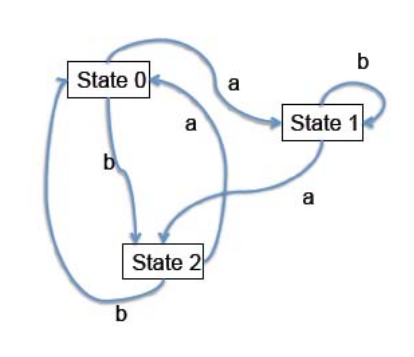
\includegraphics[width=0.4\textwidth]{img/finite-state-machine.png}
\end{center}

By monoid map we probably mean a monoid homomorphism which preserves the monoid
properties, like $f(a * b) \mapsto f(a) *' f(b)$ where $*$ is a monoid
operation. So e.g.  $2 \mapsto [a, b, b, a, b, b]$.

\begin{center}
\begin{tabular}{|c||c|}
\hline
\multicolumn{2}{|c|}{Actions} \\
\hline
$\N$ & 1 \\
\hline
State 0& State 1\\
\hline
State 1& State 2\\
\hline
State 2& State 0\\
\hline
\end{tabular}
\end{center}

For other number $n \in \N$ just apply the above tables recursively for $1 +
(n-1)$ until we reach $0 \mapsto []$.

\subsection{Groups}

\exercise{3.2.1.7}

Let \( S \) be a finite set. A permutation of \( S \) is an isomorphism \( f : S
\to S \).

\begin{center}
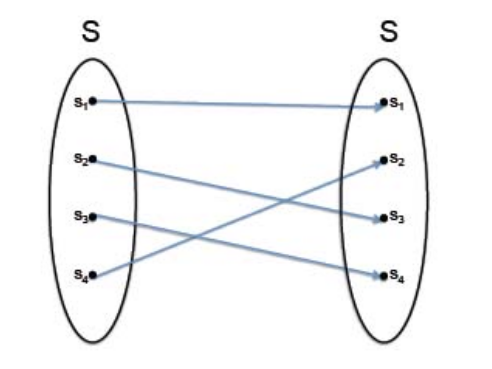
\includegraphics[width=0.4\textwidth]{img/ex3217.png}
\end{center}

\es Come up with an identity, and a multiplication formula, such that the set of
    permutations of \( S \) forms a monoid.
\ei Is it a group?
\ee

\ans

\es The identity is the identity function $f = id_S$. The multiplication is the
    function composition operator $\circ$.
\ei Yes, it is a group, because for every permutation we can define a reverse
    permutation, so $f^{-1} \circ f = id_S$.
\ee

\exercise{3.2.1.8}

In Exercise 3.1.1.27 you classified the cyclic monoids. Which of them are groups?

\ans

Cyclic monoids are characterized by two parameters: the length of their "tail"
and the length of their "cycle." A monoid is a group if its "tail" length is
zero.

\exercise{3.2.1.11}

Let \( X \) be a set and consider the group of permutations of \( X \) (see
Exercise 3.2.1.7), which we will denote \(\Sigma_X\). Find a canonical action of
\(\Sigma_X\) on \( X \).

\ans

The canonical action is just application of the permutation to the set. The
action is canonical because it follows directly from the definition of the
Group.

\exercise{3.2.1.14}

\es Consider the \( U(1) \) action on \( \Rat^3 \) given in Example 3.2.1.10.
    Describe the set of orbits of this action.
\ei What are the orbits of the action of the permutation group
    \(\Sigma_{\{1,2,3\}}\) on the set \(\{1, 2, 3\}\)? (See Exercise 3.2.1.11.)
\ee

\ans

\es The $U(1)$ action rotates points around the $Z$ axis in $\Rat^3$. So the set
    of orbits consists of the circles centered at the $Z$ axis.
\ei The permutation group action orbits are permutations of the set $S$ because
    we can set $S$ to any of its permutations using the action.
\ee

\exercise{3.2.1.15}

Let \( G \) be a group and \( X \) a set on which \( G \) acts by \(
\circlearrowright : G \times X \to X \). Is "being in the same orbit" an
equivalence relation on \( X \)?

\ans

Yes, it is. It is a reflexive, symmetrical and transitive relation.

\subsection{Graphs}

\exercise{3.3.1.4}

(a) Draw the graph corresponding to a graph tables. (b) Write down graph tables
corresponding to a graph.

\ans

\es \ 

\begin{center}
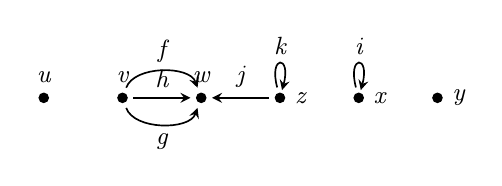
\begin{tikzpicture}
  % Define styles
  \tikzstyle{node} = [circle, draw, fill=black, inner sep=1.2pt]
  \tikzstyle{edge} = [->, semithick, shorten >=2pt, shorten <=2pt, >=stealth]

  % Nodes
  \node[node, label=above:{\small\itshape u}] (u) at (0,0) {};
  \node[node, label=above:{\small\itshape v}] (v) at (1,0) {};
  \node[node, label=above:{\small\itshape w}] (w) at (2,0) {};
  \node[node, label=right:{\small\itshape z}] (z) at (3,0) {};
  \node[node, label=right:{\small\itshape x}] (x) at (4,0) {};
  \node[node, label=right:{\small\itshape y}] (y) at (5,0) {};

  % Edges with defined style
  \draw[edge, bend left=70] (v) to node[above] {\small\itshape f} (w);
  \draw[edge, bend right=70] (v) to node[below] {\small\itshape g} (w);
  \draw[edge] (v) -- node[above] {\small\itshape h} (w);
  \draw[edge] (x) edge[loop above] node[above] {\small\itshape i} (w);
  \draw[edge] (z) -- node[above] {\small\itshape j} (w);
  \path[edge] (z) edge[loop above] node[above] {\small\itshape k} (z);
\end{tikzpicture}
\end{center}

\ei (Obvious)
\ee


\exercise{3.3.1.5}

Let \( A = \{1, 2, 3, 4, 5\} \) and \( B = \{a, b, c\} \). Draw them and
choose an arbitrary function \( f : A \to B \) and draw it. Let \( A \sqcup B \)
be the coproduct of \( A \) and \( B \) (Definition 2.4.2.1)
and let \( A \to A \sqcup B \leftarrow B \) be the two inclusions.
Consider the two functions \(\text{src}, \text{tgt} : A \to A \sqcup B\), where
\(\text{src} = i_1\) and \(\text{tgt}\) is the composition \( A \to B \to A
\sqcup B \).  Draw the associated graph \( (A \sqcup B, A, \text{src},
\text{tgt}) \).

\ans

\begin{center}
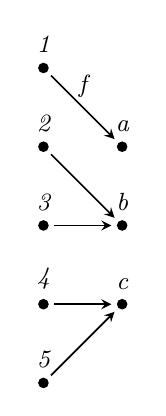
\begin{tikzpicture}
  \tikzstyle{node} = [circle, draw, fill=black, inner sep=1.2pt]
  \tikzstyle{edge} = [->, semithick, shorten >=2pt, shorten <=2pt, >=stealth]

  \node[node, label=above:{\small\itshape 1}] (1) at (1,-1) {};
  \node[node, label=above:{\small\itshape 2}] (2) at (1,-2) {};
  \node[node, label=above:{\small\itshape 3}] (3) at (1,-3) {};
  \node[node, label=above:{\small\itshape 4}] (4) at (1,-4) {};
  \node[node, label=above:{\small\itshape 5}] (5) at (1,-5) {};
  \node[node, label=above:{\small\itshape a}] (a) at (2,-2) {};
  \node[node, label=above:{\small\itshape b}] (b) at (2,-3) {};
  \node[node, label=above:{\small\itshape c}] (c) at (2,-4) {};

  \draw[edge] (1) -- node[above] {\small\itshape f} (a);
  \draw[edge] (2) -- (b);
  \draw[edge] (3) -- (b);
  \draw[edge] (4) -- (c);
  \draw[edge] (5) -- (c);
\end{tikzpicture}
\end{center}

\exercise{3.3.1.6}

\es Let $V$ be a set. Suppose we just draw the elements of $V$ as vertices and
    have no arrows between them. Is this a graph?
\ei Given $V$, is there any other “canonical” or somehow automatic non-random
    procedure for generating a graph with those vertices?
\ee

\ans

\es Yes, it is. Both its $src$ and $dst$ functions are empty sets.
\ei No, there isn't. If such a procedure existed, it would mean that a random
    set has predetermined relationships, but we know it does not.
\ee

\exercise{3.3.1.10}

Let G be the graph depicted below:

\begin{center}
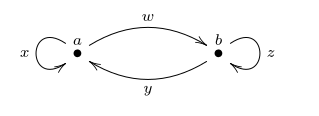
\includegraphics[width=0.4\textwidth]{img/ex33110.png}
\end{center}

Draw (using ellipses "$\ldots$" if necessary) the graph $T(G)$ defined in Example
3.3.1.9.

\ans

The answer is something like the following:

\begin{center}
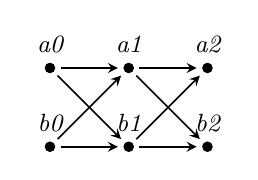
\begin{tikzpicture}
  \tikzstyle{node} = [circle, draw, fill=black, inner sep=1.2pt]
  \tikzstyle{edge} = [->, semithick, shorten >=2pt, shorten <=2pt, >=stealth]

  \node[node, label=above:{\small\itshape a0}] (a0) at (0,-1) {};
  \node[node, label=above:{\small\itshape b0}] (b0) at (0,-2) {};
  \node[node, label=above:{\small\itshape a1}] (a1) at (1,-1) {};
  \node[node, label=above:{\small\itshape b1}] (b1) at (1,-2) {};
  \node[node, label=above:{\small\itshape a2}] (a2) at (2,-1) {};
  \node[node, label=above:{\small\itshape b2}] (b2) at (2,-2) {};

  \draw[edge] (a0) -- (a1);
  \draw[edge] (b0) -- (b1);
  \draw[edge] (a1) -- (a2);
  \draw[edge] (b1) -- (b2);
  \draw[edge] (a0) -- (b1);
  \draw[edge] (b0) -- (a1);
  \draw[edge] (a1) -- (b2);
  \draw[edge] (b1) -- (a2);
\end{tikzpicture}
\end{center}

\exercise{3.3.1.11}

Consider the infinite graph $G = (V, A, \text{src}, \text{tgt})$ depicted below,

\begin{center}
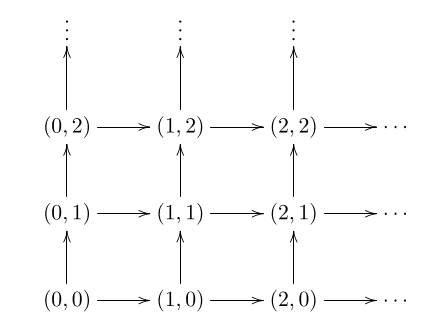
\includegraphics[width=0.4\textwidth]{img/ex33111.png}
\end{center}

\es Write down the sets $A$ and $V$.
\ei What are the source and target functions $A \to V$?
\ee

\ans

\es $V = \N \times \N$; $A = (\N \times \N) \sqcap \set{N,E}$
\ei $src = \pi_1$ so $((x,y),..) \mapsto (x,y)$;
    $dst = \set{ ((x,y),N) \mapsto (x,y+1)} \cup \set{ ((x,y),E) \mapsto
    (x+1,y)}$ where $x,y \in \N$.
\ee

\exercise{3.3.1.12}

A graph is a pair of functions $A \toto V$. This sets up the notion of
equalizer and coequalizer (see Definitions 2.5.3.1 and 2.6.3.1).

\es What feature of a graph is captured by the equalizer of its source and
    target functions?
\ei What feature of a graph is captured by the coequalizer of its source and
    target functions?
\ee


\ans

Notes:

\ls Let $f,g: X \to Y$.

\li The equalizer of $f$ and $g$ is $Eq(f,g) := \set{x \in X | f(x) = g(x)}
    \subseteq X$.

\li The coequalizer of $f$ and $g$ is $Coeq(f,g) := Y / f(x) \sim
    g(x)$ i.e.  the coequalizer of f and g is the quotient of Y by the
    equivalence relation generated by $\set{(f(x),g(x)) | x \in X} \subseteq Y
    \times Y$
\le

\es $Eq(src,dst)$ are edges that are loops (the source vertex matches the
    destination vertex).
\ei $Coeq(src,dst)$ is the relation that represents connected vertices.
\ee

\exercise{3.3.2.3}

How many paths are there in the following graph? ($V=\set{1,2,3}$,
$A=\set{f,g}$. $f$ goes from $1$ to $2$, $g$ goes from $2$ to $3$).

\ans

There are 6 paths: 3 of length 0, 2 of length 1 and 1 of length 2.

\exercise{3.3.2.4}

Let $G$ be a graph and consider the set $Path_G$ of paths in $G$. Suppose
someone claimed that there is a monoid structure on the set $Path_G$, where the
multiplication formula is given by concatenation of paths. Are they correct? Why
or why not? Hint: what should be the identity element?

\ans

No, because the monoid $(M,e,*)$ should have $*:M \times M\to M$ defined for any
element. It is not the case for path concatenation.

\exercise{3.3.3.4}

\es Where are $a, b, c, d, e$ sent under $f_1 : A \to A'$ in Diagram (3.7)?
\ei Choose a couple of elements of $A$ and check that they behave as specified
    by Diagram (3.6).
\ee

\begin{center}
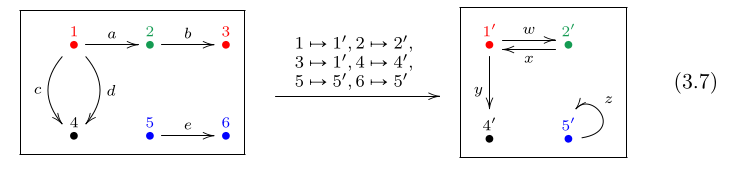
\includegraphics[width=0.8\textwidth]{img/graph-homomorphism.png}
\end{center}

\ans

\es To $w, x, y, y, z$ correspondingly.
\ei We need to check that $f_0: V \to V'$ and $f_1:A \to A'$ commute with $src$
    and $dst$ functions of both graphs. Indeed, $f_0(src(e)) = 5' =
    src'(f_1(e))$.
\ee

\exercise{3.3.3.5}

Let $G$ be a graph, let $n \in N$ be a natural number, and let $[n]$ be the
chain graph of length $n$, as in Example 3.3.1.8. Is a path of length $n$ in $G$
the same thing as a graph homomorphism $[n] \to G$, or are there subtle
differences? More precisely, is there always an isomorphism between the set of
graph homomorphisms $[n] \to G$ and the set $Path_G^{(n)}$ of length-$n$ paths
in $G$?

\ans

Note: We proof isomorphism between $A$ and $B$ by showing $(f:A\to B) \circ (g:B
\to A) = id_B$ and $g \circ f = id_A$.

Consider a set of graph homomorphisms $H = [n] \to G$. It has the following structure:
$(f_0, f_1) = (\set{0_v \mapsto v_0, 1_V \mapsto v_1, ...}, \set{0_A \mapsto
a_1, 1_A \mapsto a_2, ...})$ where $i_V$,$i_A$ - vertices and arrows of $[n]$
and $v_i$, $a_i$ - vertices and arrows of $G$.

We define $f: Path^{(n)} \to H$ and $g:H \to Path^{(n)}$ as follows: $f = v
(a_i)^{[n-1]} \mapsto (\set{i_V \mapsto v(a_i)^{[i]}}, \set{i_A \mapsto a_i})$, $g
= (\set{...}, \set{...}) \mapsto v(a_i)^{[n-1]}$ where $(a_i)^{[n]} = a_0 a_1 ...
a_{(n-1)}$, $(a_i)^0$ expands to nothing (no arrows), $n \in \set{1,...}$ -
number of path vertices.

(sounds pretty obvious that $f\circ g = id = g \circ f$)

TODO?


\exercise{3.3.3.6} Given a morphism of graphs $f : G \to G'$, there is an
induced function $\text{Path}(f) : \text{Path}(G) \to \text{Path}(G')$.

\es Is it the case that for every $n \in \mathbb{N}$, the function
    $\text{Path}(f)$ carries $\text{Path}^{(n)}(G)$ to $\text{Path}^{(n)}(G')$,
    or can path lengths change in this process?
\ei Suppose that $f_0$ and $f_1$ are injective (meaning no two distinct vertices in
    $G$ are sent to the same vertex, respectively for arrows, under $f$). Does this
    imply that $\text{Path}(f)$ is also injective (meaning no two distinct paths are
    sent to the same path under $f$)?
\ei Suppose that $f_0$ and $f_1$ are surjective (meaning every vertex in $G'$ and
    every arrow in $G'$ is in the image of $f$). Does this imply that
    $\text{Path}(f)$ is also surjective? \textit{Hint}: at least one of the
    answers to these three questions is "no".
\ee


\ans

\es Yes.
\ei Yes.
\ei No. $\text{Path}(f)$ Graph $G$ can acquire a loop, so the set of paths in
    $G'$ can become infinitely large.
\ee


\exercise{3.3.3.7}

Given a graph $(V, A, \textit{src}, \textit{tgt})$, let $i : A \to V \times V$
be the function guaranteed by the universal property for products, as applied to
$\textit{src}, \textit{tgt} : A \to V$. One might hope to summarize Condition
$(3.6)$ for graph homomorphisms by the commutativity of the single square

\begin{center}
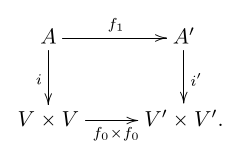
\includegraphics[width=0.25\textwidth]{img/commsquare.png}
\end{center}

Is the commutativity of the diagram in (above) indeed equivalent to the
commutativity of the diagrams in (3.6)?

\ans

I can not see reasons why the above diagram is not the equivalent of the two
diagrams in (3.6).

TODO: Need to double-check! Very interesting! Can it be related to the no-arrows
graphs? Can it be related to loop-arrows in graphs? Note: Is it about problems
with sibling arrows? Most likely yes!


\exercise{3.3.3.10}

A relation on $\Rat$ is a subset of $\Rat \times \Rat$, and one can indicate
such a subset of the plane by shading. Choose an error bound $\epsilon > 0$ and
draw the relation one might refer to as "$\epsilon$-approximation". To say it
another way, draw the relation "$x$ is within $\epsilon$ of $y$".

\ans

An ascending bar centered at the $y=x$ line, with $2*\epsilon$ height.

\exercise{3.3.3.11} (Binary relations to graphs).

\es If $R \subseteq S \times S$ is a binary relation, find a natural way to make
    a graph out of it, having vertices $S$.
\ei What is the set $A$ of arrows?
\ei What are the source and target functions $\text{src}, \text{tgt} : A \to S$?
\ei Take the left-hand table in (3.9) and consider its first $7$ rows (i.e.
    forget the $..$). Draw the corresponding graph (do you see a tetrahedron?).
\ei Do the same for the right-hand table.
\ee

\ans

\es Points go to Vertices, Points in relation go to Arrows, $src$ and $dst$ mark
    left-hand side and right-hand side points in relation.
\ei Arrows indicate points in relation to each other.
\ei $src$ selects left-hand side points in relation, $dst$ selects right-hand
    side points.
\li Graph corresponding to the left table in (3.9).

    \begin{center}
    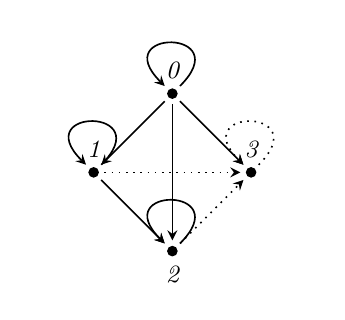
\begin{tikzpicture}
      \tikzstyle{node} = [circle, draw, fill=black, inner sep=1.2pt]
      \tikzstyle{edge} = [->, semithick, shorten >=2pt, shorten <=2pt, >=stealth]

      \node[node, label=above:{\small\itshape 0}] (0) at (0,0) {};
      \node[node, label=above:{\small\itshape 1}] (1) at (-1,-1) {};
      \node[node, label=below:{\small\itshape 2}] (2) at (0,-2) {};
      \node[node, label=above:{\small\itshape 3}] (3) at (1,-1) {};

      \draw[edge, looseness=30] (0) to (0);
      \draw[edge] (0) to (1);
      \draw[edge, looseness=30] (1) to (1);
      \draw[edge] (0) to (2);
      \draw[edge] (1) to (2);
      \draw[edge, looseness=30] (2) to (2);
      \draw[edge] (0) to (3);
      \draw[edge, dotted] (1) to (3);
      \draw[edge, dotted] (2) to (3);
      \draw[edge, dotted, looseness=30] (3) to (3);
    \end{tikzpicture}
    \end{center}
\ei Graph corresponding to the right-hand table in (3.9)
    \begin{center}
    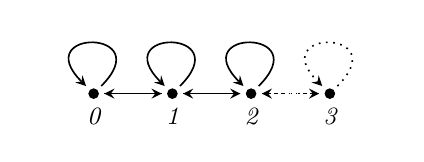
\begin{tikzpicture}
      \tikzstyle{node} = [circle, draw, fill=black, inner sep=1.2pt]
      \tikzstyle{edge} = [->, semithick, shorten >=2pt, shorten <=2pt, >=stealth]
      \node[node, label=below:{\small\itshape 0}] (0) at (0,0) {};
      \node[node, label=below:{\small\itshape 1}] (1) at (1,0) {};
      \node[node, label=below:{\small\itshape 2}] (2) at (2,0) {};
      \node[node, label=below:{\small\itshape 3}] (3) at (3,0) {};
      \draw[edge] (0) to (1);
      \draw[edge] (1) to (0); // Reverse edge
      \draw[edge] (1) to (2);
      \draw[edge] (2) to (1); // Reverse edge
      \draw[edge, dotted] (2) to (3);
      \draw[edge, dotted] (3) to (2); // Reverse edge
      \draw[edge, looseness=30] (0) to (0); // Loop
      \draw[edge, looseness=30] (1) to (1); // Loop
      \draw[edge, looseness=30] (2) to (2); // Loop
      \draw[edge, dotted, looseness=30] (3) to (3); // Loop
    \end{tikzpicture}
    \end{center}
\ee


\exercise{3.3.3.12} (Graphs to binary relations).

\ls If $(V, A, src, tgt)$ is a graph, find a natural way to make a binary
    relation $R \subseteq V \times V$ out of it.
\li Take the left-hand graph $G$ from (3.7) and write out the corresponding
    binary relation in table form.
    \begin{center}
    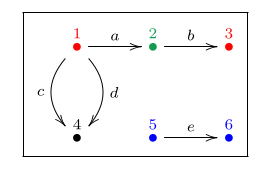
\includegraphics[width=0.25\textwidth]{img/3-7-left.png}
    \end{center}
\le

\ans

\ls Let $R_G \subseteq V \times V = \set{(src(a), dst(a)) | a \in A_G}$.
\li $R_G = \set{(1,4),(1,2),(2,3),(5,6)}$. Note: What about duplications, here
    $(1,4)$?
\le


\exercise{3.3.3.13} (Going around the loops)

\ls Given a binary relation $R \subseteq S \times S$, you know from Exercise
    3.3.3.11 how to construct a graph out of it, and from Exercise 3.3.3.12 how
    to make a new binary relation out of that. How does the resulting relation
    compare with the original?
\li Given a graph $(V, A, src, tgt)$, you know from Exercise 3.3.3.12 how to
    make a new binary relation out of it, and from Exercise 3.3.3.11 how to
    construct a new graph out of that. How does the resulting graph compare with
    the original?
\le

\ans

\ls The new relation will be identical to the original
\li The new graph will not be identical to the original. The sibling arrows will
    be joined into one arrow. The vertices without arrows will disappear.
\le

\subsection{Orders}

\exercise{3.4.1.2}

\ls Decide whether the table to the left in Display (3.9) constitutes a linear
    order.
\li Show that neither of the other tables are even preorders.
\le

\ans

\ls Yes it is a linear order. It is reflexive, transitive, antisymmetric and
    comparable.
\li The $|n-m| \leq 1$ is not transitive, thus, it is not a preorder. The $n=5m$
    relation has gaps (not reflexive), so, again, not a preorder.
\le


\exercise{3.4.1.8}

Let $S = \{1, 2, 3, 4\}$.

\es Find a preorder $R \subseteq S \times S$ such that the set $R$ is as small
    as possible. Is it a partial order? Is it a linear order?
\ei Find a preorder $R_1 \subseteq S \times S$ such that the set $R_1$ is as
    large as possible. Is it a partial order? Is it a linear order?
\ee

\ans

\es $R = \set{(1,1),(2,2),(3,3),(4,4)}$. It is reflexive, and formally
    transitive. It is a partial order. It is not a linear order.
\ei $R_1$ should be a fully-connected graph. It is a reflexive and transitive by
    definition, but it contains non-trivial loops (symmetric). Thus, it is not a
    partial order. Also it is not a linear order.
\ee

\exercise{3.4.1.9}

\es List all the preorder relations possible on the set $\set{1, 2}$.
\ei For any $n \in \N$, how many linear orders exist on the set
    $\set{1, 2, 3, \ldots, n}$.
\ei Does your formula work when $n = 0$?
\ee

\ans

\es There are $\set{(1,1),(2,2)}$, $\set{(1,1),(2,2),(1,2)}$,
    $\set{(1,1),(2,2),(2,1)}$, $\set{(1,1),(2,2),(1,2),(2,1)}$.
\ei Linear orders are permuations of set elements. Thus, for n-element set there
    are $ n! $ linear orders.
\ei $0!$  is set to be $1$, and there is one linear order $R \subseteq \set{} \times
    \set{} = \set{}$. So, the formula works.
\ee

\exercise{3.4.1.12}

Let $G = (V, A, src, tgt)$ be the graph below.

\begin{center}
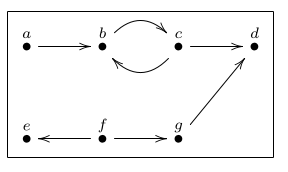
\includegraphics[width=0.25\textwidth]{img/order-example.png}
\end{center}

In the corresponding pre-order which of the following are true:

(a) $a \leq b$?
(b) $a \leq c$?
(c) $c \leq b$?
(d) $b = c$?
(e) $e \leq f$?
(f) $f \leq d$?

\ans

(a) True (b) True (c) True (d) False. The equality is a partial-order
requirement. (e) False (f) True.

\exercise{3.4.1.13}

\es Let $S = \{1, 2\}$. The subsets of $S$ form a partial order; draw the
    associated graph.
\ei Repeat this for $Q = \emptyset$, $R = \{1\}$, and $T = \{1, 2, 3\}$.
\ei Do you see $n$ - dimensional cubes?
\ee

\ans

\es $S = \{1, 2\}$:
    \begin{center}
    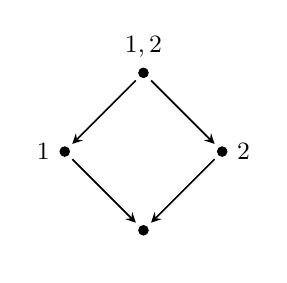
\begin{tikzpicture}
      \tikzstyle{node} = [circle, draw, fill=black, inner sep=1.2pt]
      \tikzstyle{edge} = [->, semithick, shorten >=2pt, shorten <=2pt, >=stealth]
      \node[node, label=above:{\small\itshape $\set{1,2}$}] (12) at (0,0) {};
      \node[node, label=left:{\small\itshape $\set{1}$}] (1) at (-1,-1) {};
      \node[node, label=right:{\small\itshape $\set{2}$}] (2) at (1,-1) {};
      \node[node, label=below:{\small\itshape $\set{}$}]  (0) at (0,-2) {};
      \draw[edge] (12) to (1);
      \draw[edge] (12) to (2);
      \draw[edge] (1) to (0);
      \draw[edge] (2) to (0);
    \end{tikzpicture}
    \end{center}
\ei
    $Q = \set{}$ - a dot; $R = \set{1}$ - a line; $T = \set{1,2,3}$:
    \begin{center}
    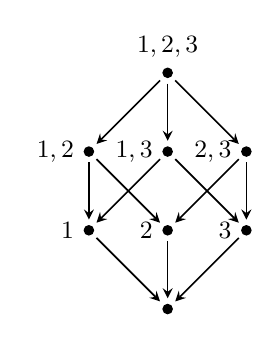
\begin{tikzpicture}
      \tikzstyle{node} = [circle, draw, fill=black, inner sep=1.2pt]
      \tikzstyle{edge} = [->, semithick, shorten >=2pt, shorten <=2pt, >=stealth]
      \node[node, label=above:{\small\itshape $\set{1,2,3}$}] (123) at (0,0) {};
      \node[node, label=left:{\small\itshape $\set{1,2}$}] (12) at (-1,-1) {};
      \node[node, label=left:{\small\itshape $\set{1,3}$}] (13) at (0,-1) {};
      \node[node, label=left:{\small\itshape $\set{2,3}$}] (23) at (1,-1) {};
      \node[node, label=left:{\small\itshape $\set{1}$}] (1) at (-1,-2) {};
      \node[node, label=left:{\small\itshape $\set{2}$}] (2) at (0,-2) {};
      \node[node, label=left:{\small\itshape $\set{3}$}] (3) at (1,-2) {};
      \node[node, label=below:{\small\itshape $\set{}$}]  (0) at (0,-3) {};
      \draw[edge] (123) to (12);
      \draw[edge] (123) to (13);
      \draw[edge] (123) to (23);
      \draw[edge] (12) to (1);
      \draw[edge] (12) to (2);
      \draw[edge] (13) to (1);
      \draw[edge] (13) to (3);
      \draw[edge] (23) to (2);
      \draw[edge] (23) to (3);
      \draw[edge] (1) to (0);
      \draw[edge] (2) to (0);
      \draw[edge] (3) to (0);
    \end{tikzpicture}
    \end{center}

\ei
    Yes
\ee

\exercise{3.4.1.15}

True or false: a partial order is a preorder that has no cliques. (If false, is
there a "nearby" true statement?)

\ans

Note: Let $(S, \leq)$ be a preorder. A clique is a subset $S' \subseteq S$ such that
for each $a, b \in S'$ one has $a \leq b$.

One-element clique are always possible and valid for pre-orders. We must say: a
partial order is a preorder that has no two- or more element cliques.

\exercise{3.4.1.17}

Let $X = \{a, b, c, d, e, f\}$ and let $R = \{(a, b), (b, c), (b, d), (d, e),
(f, a)\}$.

\es What is the preorder $\overline{R}$ generated by $R$?
\ei Is it a partial order?
\ee

\ans

Note: preopder is a binary relation which is (a) reflexive ($s \leq s`$). (b) transitive
(if $s \leq s' \land s' \leq s''$ then $s \leq s''$).

Note: $\overline{R}$ is a preorder generated by a relation $R$ if (a) $ R
\subseteq \overline{R}$. (b) $\overline{R}$ is reflexive (c) $\overline{R}$ is
transitive.

\es Graph of $R$ looks like a ring so $\overline{R}$ is a full graph.
\ei It is not a partial order because there are loops in full graphs.
\ee

\exercise{3.4.1.18}

Let $X$ be the set of people and let $R \subseteq X \times X$ be the relation
with $(x, y) \in R$ if $x$ is the child of $y$. Describe the preorder generated
by $R$.

\ans

$\overline{R}$ is an ancestry relation. $(x,y) \in \overline{R}$ if $y$ is an
ancestor of $x$.

\exercise{3.4.2.2}

Consider the partial order from Example 3.4.1.3.

\es What is the join of $(\text{a diamond})$ and $(\text{a heart})$?
\ei What is the meet of $(\text{a black card})$ and $(\text{a queen})$?
\ei What is the meet of $(\text{a diamond})$ and $(\text{a card})$?
\ee

\ans

Note: meet is a maximum lower bound. join is a minimum upper bound. meets and
joins are defined on a preorder.

Note: In example 3.4.1.3 $A \to B$ means $A \leq B$.

\es Join of "a diamond" and "a heart" is "a red card".
\ei Meet of "a black card" and "a queen" is "a black queen".
\ei Meet of "a diamond" and "a card" is "a diamond" itself.
\ee

\exercise{3.4.2.3}

\es If possible, find two elements in the partial order from Example 3.4.1.3
    that do not have a meet.
\ei If possible, find two elements that do not have a join (in that preorder).
\ee

\ans

\es "a diamond" and "a heart" don't have a meet
\ei Every element of this preorder has a join, often it is "a card".
\ee

\exercise{3.4.2.4}

As mentioned in the introduction to this section, the power set $S :=
\mathcal{P}(X)$ of any set $X$ naturally has the structure of a partial order.
Its elements $s \in S$ correspond to subsets $s \subseteq X$, and we put $s \leq
t$ if and only if $s \subseteq t$ as subsets of $X$. The meet of two elements is
their intersection as subsets of $X$, $s \wedge t = s \cap t$, and the join of
two elements is their union as subsets of $X$, $s \vee t = s \cup t$.

\es Is it possible to put a monoid structure on the set $S$ in which the
    multiplication formula is given by meets? If so, what would the identity
    element be?
\ei Is it possible to put a monoid structure on the set $S$ in which the
    multiplication formula is given by joins? If so, what would the identity
    element be?
\ee

\ans

Note: Monoid structure $(M,e,*)$ requires the following properties: (1) Left-Identity (2)
Right-Identity (3) Associativity

\es Yes. The identity is the full set $S$, so (1) $S \wedge a = a$, (2) $a \wedge S = a$,
    (3) $a \wedge (b \wedge c) = (a \wedge b) \wedge c$.
\ei Yes. The identity is the empty set $\emptyset$.
\ee

\exercise{3.4.2.6}

Consider the tree drawn in (3.11).

\begin{center}
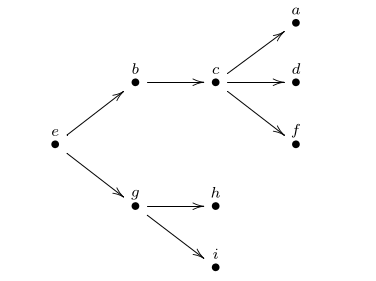
\includegraphics[width=0.4\textwidth]{img/a-tree.png}
\end{center}

\es What is the meet $i \wedge h$?
\ei What is the meet $h \wedge b$?
\ei What is the join $b \vee a$?
\ei What is the join $b \vee g$?
\ee

\ans

\es $g = i \wedge h$.
\ei $e = h \wedge b$.
\ei $a = b \vee a$.
\ei $b$ and $g$ have no join.
\ee

\vsp
\vsp
\vsp
\vsp

\printbibliography

\end{document}

